% quantum_vina_qst.tex
% Quantum Science and Technology (IOP) -- iopjournal class
% Skeleton built 4 September 2026. Every %% TODO marks a fact that is not
% yet resolved in the verified record; do not delete a TODO without the
% source value in hand.

\PassOptionsToPackage{hypertexnames=false}{hyperref}
\documentclass{iopjournal}

% ---------------------------------------------------------------------
% Packages (iopjournal ships none of these; all are standard TeX Live)
% ---------------------------------------------------------------------
\usepackage{amsmath,amssymb}
\usepackage{booktabs}
\usepackage{tabularx}
\usepackage{graphicx}
\usepackage{siunitx}
\DeclareSIUnit\angstrom{\text{\AA}}
\usepackage{algorithm}
\usepackage{algpseudocode}
\usepackage{xcolor}
\usepackage{hyperref}

\graphicspath{{figures/}}

% Placeholder macro: renders a visible box so unresolved values cannot ship silently
\newcommand{\todo}[1]{\textcolor{red}{[TODO: #1]}}
% Placeholder figure box, fixed height, until the real file exists.
% Replace \placeholderfig{name}{h} with \includegraphics[width=...]{name} when ready.
\newcommand{\placeholderfig}[2]{\fbox{\parbox[c][#2][c]{0.8\textwidth}{\centering\textcolor{red}{figure placeholder: \texttt{\detokenize{#1}}}}}}

% Fixed notation
\newcommand{\ket}[1]{\left|#1\right\rangle}
\newcommand{\Hc}{H_{\mathrm{C}}}
\newcommand{\Hm}{H_{\mathrm{M}}}
\newcommand{\AR}{\mathrm{AR}}

\begin{document}

\articletype{Paper}

\title{Penalty formulation and instance size determine what a QAOA docking hardware result reveals: a two-campaign study on IBM Heron processors}
%% TODO title: candidate only, pending Suriya's approval; the previous title described the pre-reframing paper.

\author{Suriya Narayanan Rajavel$^{1}$\orcid{0009-0003-2590-0099}}

\affil{$^1$Independent researcher, San Jose, California, United States of America}

\email{suriyarajavel02@gmail.com}

\keywords{molecular docking, maximum weighted clique, quantum optimization, QAOA, QUBO, penalty formulation, approximation ratio, superconducting quantum processors, NISQ, reproducibility}

% =====================================================================
\begin{abstract}
Molecular docking can be cast as a maximum weighted clique problem on a pharmacophore compatibility graph, and hardware executions of the quantum approximate optimization algorithm (QAOA) on such instances have begun to appear. This paper asks what such a result reveals about the formulation it executed, and which reported quantities can reveal it. Eleven-node instances built from AutoDock Vina-GPU 2.1 poses of human $\beta$II tryptase (PDB 2BM2) and HIV-1 protease with indinavir (PDB 1HSG) were executed on two IBM Heron processors, five runs of 4096 shots each, with a penalty of half the largest node weight, below the condition that guarantees a feasible ground state; on 2BM2 the ground state was infeasible. The heaviest valid sample nonetheless matched the brute-force optimum in every run, and that outcome is shown to have been guaranteed at these shot counts under uniform sampling within the feasible set. Reconstructing every executed Hamiltonian from the submitted circuits and recomputing every statistic from the raw counts, the paper reports two quantities that do discriminate, the concentration on the optimum relative to uniform feasible sampling and the feasibility of the sampled mode, and three controlled re-executions on the same graphs and devices, 280 further jobs, that vary the penalty, the depth and the instance size. The formulation error is visible at every depth on three-node instances and invisible at depth one on eleven nodes; the transition lies above eight nodes on both graphs, and the depth-one mode follows the penalty-to-weight ratio and the instance size rather than the location of the ground state. A calibration-based noise model reproduces both devices up to about 100 two-qubit gates and, beyond that, one device but not the other.
\end{abstract}

% =====================================================================
\section{Introduction}
\label{sec:intro}

The cost of bringing a new medicine to market has been estimated at \$2.6 billion per approved compound in 2013 dollars when capitalised over the failures that precede each success~\cite{dimasi2016cost}, and at a median of \$1.1 billion and a mean of \$1.6 billion in 2018 dollars from a different sample and a different treatment of failed candidates~\cite{wouters2020cost}. Whichever figure is preferred, a substantial share of it is spent before any compound reaches an assay, in the stage where candidate molecules are selected from libraries that now exceed one hundred million entries; a single 2019 campaign docked 99 million compounds against one target and 138 million against another~\cite{lyu2019ultralarge}. Structure-based virtual screening reduces this expense by predicting, from the three-dimensional structure of the target, how each candidate binds within the protein pocket, so that only the most promising compounds proceed to synthesis. The prediction step is molecular docking, and its accuracy determines which candidates are carried forward and which are discarded.

Docking engines such as AutoDock Vina and its GPU-accelerated derivatives~\cite{trott2010vina,tang2022vinagpu,ding2023vinagpu2,tang2024vinagpu21} search a continuous space of ligand positions, orientations and torsions under an empirical scoring function and return a ranked set of binding poses. An alternative, discrete view of the same problem was introduced by Kuhl \textit{et al}~\cite{kuhl1984combinatorial}, following earlier geometric matching approaches~\cite{kuntz1982geometric}. Protein and ligand are each reduced to a small set of pharmacophores, every candidate protein--ligand pairing becomes a node, two nodes are joined by an edge when their contacts can be satisfied at the same time, and a physically consistent binding mode corresponds to a clique. Selecting the highest-weight clique is a combinatorial optimization problem in which the number of candidate contact sets grows exponentially with the number of nodes: an instance with eleven candidate contacts already has 2048 subsets, of which only the mutually compatible ones are admissible. This formulation is what has made docking a recurring test case for quantum optimization.

Recent advances in quantum computing have motivated the investigation of quantum optimization methods for combinatorial problems of this kind~\cite{preskill2018nisq,farhi2014qaoa}, and graph-based docking has been addressed on photonic, annealing, neutral-atom and gate-model platforms, most of the latter in simulation~\cite{banchi2020gbs,triuzzi2025weighted,garrigues2026scalable,ding2024docking,papalitsas2025qaoa}. Two gate-model hardware executions appeared in July and August 2026, on an IBM Eagle processor~\cite{zheng2026qscore} and on an IBM Heron processor~\cite{chen2026fbe}. As section~\ref{sec:related} details, these studies report the quality of the best feasible sample and, at most, one execution per instance; none reports whether the formulation's ground state was feasible, whether the sampled mode was, or how the reported quantity compares with sampling uniformly over the feasible set. Those are the questions this paper asks of its own experiment.

The objective of this work is to establish what a QAOA docking result obtained on current superconducting hardware reveals about the formulation it executed, and which reported quantities are able to reveal it. A docked pose produced by AutoDock Vina-GPU 2.1 is reduced to a pharmacophore compatibility graph, the maximum weighted clique on that graph is formulated as a QUBO model, and the resulting circuits were executed on IBM Heron processors for two published protein--ligand complexes in July 2026. The formulation used a penalty below the condition required for a feasible ground state. Rather than discard the record, the paper reconstructs the executed instances from the submitted circuits, recomputes every statistic from the raw counts, and adds three controlled re-executions on the same graphs and devices that vary the penalty, the depth and the instance size.

The primary contributions of this work are:
\begin{enumerate}
\item A reconstruction method for executed QAOA instances. From a submitted depth-one circuit the edge set, the relative weights, the penalty-to-weight ratio and the optimum are recovered exactly, up to a bit-complement ambiguity that the angle grid resolves, and from a submitted circuit of any depth its noiseless output distribution. Applied to the July record it identified a penalty of half the largest weight, an infeasible ground state on one target, and a bit-order error that had invalidated every per-run statistic in the original analysis.
\item A demonstration that the approximation ratio reported for such experiments carries no information at realistic shot counts: with 37 feasible strings and several hundred feasible shots the optimum is observed with probability $1 - 10^{-6}$ under uniform sampling, so a ratio of 100\% was guaranteed for the defective formulation. Two quantities that do discriminate, the concentration on the optimum relative to uniform-within-feasible sampling and the feasibility of the sampled mode, are defined and reported throughout.
\item Controlled re-executions on the same graphs and devices that locate when the formulation error is visible: at every depth on three-node instances, not at depth one on the eleven-node 2BM2 instance, with the executed penalty's signature present in every run at eight nodes and below on both graphs and the corrected penalty crossing in the opposite direction above eight nodes on both. At depth one the sampled mode follows the penalty-to-weight ratio and instance size rather than the location of the ground state, as measured on a five-node subgraph whose ground state is feasible under the executed penalty; at depth three, with well-optimized angles, it follows the ground state.
\item Two auxiliary findings needed to interpret the above: the expectation-optimal angles are part of the result, since angles from different grids on one Hamiltonian give different feasibility behaviour; and a calibration-based noise model reproduces both devices to within 0.03 up to about 100 two-qubit gates, beyond which it under-predicts the degradation of \texttt{ibm\_marrakesh}, where the July 2BM2 decomposition ran, while continuing to reproduce \texttt{ibm\_fez} to 164 two-qubit gates.
\end{enumerate}

The instances considered are small enough to be solved by exhaustive classical enumeration, which serves as the reference throughout; nothing in the paper bears on quantum advantage. The contribution is a method for auditing a hardware record and a set of measured conditions under which a common class of formulation error is, and is not, detectable in QAOA output.

The remainder of the paper is organized as follows. Section~\ref{sec:related} reviews classical docking and quantum approaches to docking. Section~\ref{sec:inputs} describes the two targets, the docking inputs and the pharmacophore graph. Section~\ref{sec:formulation} presents the QUBO and Ising formulations as executed and the corrected penalty, and section~\ref{sec:methods} the QAOA circuits, the parameter selection and the recombination step. Section~\ref{sec:setup} describes the two campaigns, the reconstruction of executed instances and the analysis conventions, and section~\ref{sec:results} presents the results experiment by experiment. Finally, sections~\ref{sec:discussion} and~\ref{sec:conclusion} discuss the findings and conclude the paper.
%% NOTE: ~720 words of prose against a 600 budget after the paragraph-3 trim.
%% "Past two months" must be updated at submission.

% =====================================================================
\section{Related work}
\label{sec:related}
%% Verified facts (4 Sep 2026 sweep) that govern this section:
%% Zheng 2026: ibm_rensselaer (Eagle r3); 6 AND 10 qubits on hardware; 1000
%%   circuits = 250 molecules x 4 configurations, so one execution per
%%   instance-configuration (inferred, not stated); GNN orbital graph; Vina used
%%   only as a classical baseline scorer, not as the graph source.
%% Chen 2026: ibm_kingston (Heron r2); FBE, 6 qubits for 18 variables and 5 for
%%   14; pharmacophores from PDB structures per Ding's criteria (NetworkX,
%%   PyMOL); 1000 repetitions in SIMULATION; hardware repetitions not stated.
%% Ding 2024: <=12 nodes, ma-DC-QAOA, MindQuantum simulation. Papalitsas 2025:
%%   14 and 17 nodes, GPU simulation, no QPU. Garrigues 2026: emu-sv emulation,
%%   MWIS on the complement graph (= MWC). Cazals 2025: Orion-alpha, random graphs.
%% Triuzzi 2025, Micucci 2026: real D-Wave, ligands <= 6 heavy atoms, low valid
%%   yields. Yu 2023: 32-node clique on photonic hardware is a constructed graph.
%% Gap wording: "none builds the graph from the pose returned by a production
%%   docking engine, with the partial exception of Zheng (Vina as baseline scorer)";
%%   "run-to-run variability not characterized: one execution per configuration
%%   or repetitions not stated".

The literature relevant to this work spans four areas, reviewed in turn below: docking within structure-based drug discovery (section~\ref{sec:rel-sbdd}), the AutoDock Vina lineage (section~\ref{sec:rel-vina}), quantum docking on annealing, photonic and neutral-atom platforms (section~\ref{sec:rel-other}), and quantum docking on gate-model processors (section~\ref{sec:rel-gate}).

\subsection{Molecular docking in structure-based drug discovery}
\label{sec:rel-sbdd}
Structure-based drug discovery uses the three-dimensional structure of a protein target to select and refine candidate ligands, and docking is the step in which each candidate is placed within the binding pocket and scored~\cite{trott2010vina}. The scale of the task has grown with the libraries: ultra-large campaigns now dock on the order of one hundred million make-on-demand compounds against a single target~\cite{lyu2019ultralarge}, so the cost of the docking step is a direct multiplier on the cost of screening. The discrete formulation used in this paper, in which docking is expressed as the search for a maximum weighted clique on a graph of candidate protein--ligand contacts, was introduced by Kuhl \textit{et al}~\cite{kuhl1984combinatorial}, following earlier geometric matching approaches~\cite{kuntz1982geometric}. The present work uses the continuous engine to produce the pose and the discrete graph to optimize the contact set; the engine is described next.

\subsection{Classical docking and the Vina lineage}
\label{sec:rel-vina}
AutoDock Vina~\cite{trott2010vina} searches the space of ligand positions, orientations and torsion angles with a Monte Carlo procedure under an empirical scoring function and reports improved binding-mode prediction relative to AutoDock 4. Its successors extend the program rather than the method: Vina 1.2 adds force fields and Python bindings~\cite{eberhardt2021vina12}; Vina-GPU~\cite{tang2022vinagpu} and Vina-GPU 2.0~\cite{ding2023vinagpu2} move the search onto graphics processors; and Vina-GPU 2.1~\cite{tang2024vinagpu21}, the version used here, further reduces docking time while retaining Vina's scoring function. The output of any member of this lineage is a set of ranked poses with scores, and it is this output, not the crystal structure, that the present pipeline takes as its input.

\subsection{Quantum docking on annealing, photonic and neutral-atom platforms}
\label{sec:rel-other}
Banchi \textit{et al}~\cite{banchi2020gbs} recast the maximum weighted clique on a binding interaction graph as a Gaussian boson sampling problem, and Yu \textit{et al}~\cite{yu2023gbs} executed it on programmable photonic hardware, although the largest clique instance in that demonstration is a constructed 32-node graph rather than a docking instance. On quantum annealers, Triuzzi \textit{et al}~\cite{triuzzi2025weighted} and Micucci \textit{et al}~\cite{micucci2026subgraph} formulate docking as weighted subgraph isomorphism and execute it on D-Wave hardware for ligands of at most six heavy atoms, reporting low yields of valid solutions; Beneventi \textit{et al}~\cite{beneventi2026pistacking} extend the same QUBO formulation with a $\pi$-stacking term, evaluated with simulated annealing. On neutral-atom processors the problem is posed as a maximum weighted independent set on the complement graph, which is equivalent to the clique problem; Garrigues \textit{et al} studied it first for small instances~\cite{garrigues2024towards} and then with the divide-and-conquer heuristic of Cazals \textit{et al}~\cite{cazals2025rydberg}, entirely in emulation~\cite{garrigues2026scalable}. Cazals \textit{et al} did execute that heuristic on Pasqal's Orion-$\alpha$ processor, but on random graphs, not docking instances.

\subsection{Quantum docking on gate-model processors}
\label{sec:rel-gate}
For gate-model devices the Quantum Approximate Optimization Algorithm is the standard route. Ding \textit{et al}~\cite{ding2024docking} introduced a digitized-counterdiabatic QAOA for the clique formulation and evaluated it in simulation at up to twelve nodes; Papalitsas \textit{et al}~\cite{papalitsas2025qaoa} extended the approach with warm starts to fourteen- and seventeen-node instances, again in simulation on a GPU cluster. Two hardware studies appeared in July and August 2026. Zheng \textit{et al}~\cite{zheng2026qscore} build the contact graph from orbital interaction energies predicted by a graph neural network, solve it with digitized-counterdiabatic QAOA, and execute 1000 circuits on the IBM Eagle processor \texttt{ibm\_rensselaer} at six and ten qubits, with the ten-qubit configurations described as noise-limited; the circuit count corresponds to one execution per molecule and configuration, and Vina is used only as a classical baseline scorer. On the adjacent problem of hydration-site prediction, Loco \textit{et al}~\cite{loco2025hydration} execute a QUBO formulation on IBM Heron processors at up to 123 qubits and report the result as agreement of the decoded answer with a classical reference; a later review from the same group~\cite{ansari2026convergence} places that work in the context of hybrid quantum--classical drug discovery. Chen \textit{et al}~\cite{chen2026fbe} take pharmacophores directly from the PDB structures following the criteria of Ding \textit{et al}, and execute a variational full-basis encoding on the IBM Heron processor \texttt{ibm\_kingston}, representing eighteen contact variables with six qubits in one test and fourteen with five in the other; the number of hardware repetitions is not stated. Table~\ref{tab:related} summarizes these studies alongside the present work.

Across these studies the hardware result is reported as the quality of the best feasible sample, or as agreement of the decoded answer with a classical calculation, from one execution per instance or an unstated number. None reports whether the penalty of its formulation satisfied the feasibility condition, whether the ground state of the executed Hamiltonian was feasible, what the sampled mode was, or how the reported quantity compares with sampling uniformly over the feasible set. On instances small enough to enumerate, and every instance above is, those are the quantities that determine whether the reported success says anything about the circuit. The present work asks them of its own July 2026 execution, which turns out to have carried a defective penalty, and uses re-executions on the same devices to establish when such a defect is visible.

\begin{table}[htbp]
\caption{Comparison with prior quantum docking studies. MWC: maximum weighted clique; MWVC/MVWCP: maximum weighted vertex clique; MWIS: maximum weighted independent set (on the complement graph, equivalent to MWC); FBE: full-basis encoding; n.s.: not stated. $^{\dagger}$Inferred from 250 molecules $\times$ 4 configurations $=$ 1000 circuits; not stated by the authors.}
\label{tab:related}
\centering
\footnotesize
\begin{tabularx}{\textwidth}{@{}>{\raggedright\arraybackslash}p{2.6cm} l l >{\raggedright\arraybackslash}X c c >{\raggedright\arraybackslash}X@{}}
\toprule
Work & Problem & Solver & Platform & Qubits & Runs & Classical front end \\
\midrule
Ding 2024 \cite{ding2024docking} & MWC & DC-QAOA & simulation & $\le 12$ & -- & -- \\
Papalitsas 2025 \cite{papalitsas2025qaoa} & MWC & DC-QAOA & GPU simulation & 14, 17 & -- & -- \\
Zheng 2026 \cite{zheng2026qscore} & MWVC & DC-QAOA & IBM Eagle r3 & 6, 10 & 1$^{\dagger}$ & GNN orbital graph \\
Chen 2026 \cite{chen2026fbe} & MVWCP & FBE & IBM Heron r2 & 5--6 & n.s. & none (PDB pharmacophores) \\
Garrigues 2026 \cite{garrigues2026scalable} & MWIS & analog annealing & emulator (emu-sv) & 225--585 nodes, in emulated subgraphs & grid search & RDKit \\
This work & MWC & QAOA + decomp. & IBM Heron, 2 devices & 11 & 5 & Vina-GPU 2.1 \\
\bottomrule
\end{tabularx}
\end{table}

% =====================================================================
\section{Inputs and docking problem setup}
\label{sec:inputs}

The quantum optimization study reported in this paper takes as its input the docked poses produced by a classical docking engine for two published protein--ligand complexes. This section describes the two targets, the docking step, the reduction of each pose to a small set of pharmacophores, and the compatibility graph on which the optimization is defined. The contribution of the paper lies in the formulation, execution and analysis of the graph problem on quantum hardware; the docking engine and the crystal structures are used as fixed inputs.

\subsection{Targets}
\label{sec:targets}
Two complexes were selected from the Protein Data Bank. The first is human $\beta$II tryptase in complex with a 4-(3-aminomethylphenyl)piperidinyl-1-amide inhibitor (PDB 2BM2)~\cite{levell2005tryptase}, a trypsin-like serine protease released during mast-cell activation. The second is HIV-1 protease in complex with indinavir (PDB 1HSG, ligand code MK1)~\cite{chen1994hsg}, a standard benchmark complex in the docking literature. The two produce compatibility graphs of the same size but different density, and that difference is used throughout the paper as a control.

\subsection{Classical docking}
\label{sec:vina}
Each ligand was docked into its receptor with AutoDock Vina-GPU 2.1~\cite{tang2024vinagpu21}, the GPU implementation of the Vina scoring function~\cite{trott2010vina}, with the search box centred on the crystal-ligand centroid, a box edge of \SI{20}{\angstrom}, exhaustiveness 8 and nine output modes. The top-ranked pose was used as the input to the pharmacophore extraction; the crystal pose was not used beyond defining the box. Reference scores of \SI{-8.98}{kcal/mol} (2BM2) and \SI{-10.54}{kcal/mol} (1HSG) were recorded. The docking runs were not seeded and the notebook that reduced the poses to graphs was not preserved in the form that was executed, so the docking step cannot be repeated to reproduce the executed graphs exactly. The paper therefore treats the executed graphs, recovered from the submitted circuits (section~\ref{sec:setup}), as authoritative: their edge sets, relative weights and optima are exact, the absolute weight scale is not used, and the docking parameters stated in this section describe the procedure as recorded rather than a reproduction of it.

\subsection{Pharmacophore extraction and selection}
\label{sec:pharma}
Pharmacophores were assigned from the AutoDock atom types in the PDBQT files as hydrogen-bond acceptors (HA), hydrogen-bond donors (HD), hydrophobic centres (HY) and aromatic centres (AR). Protein pharmacophores were collected within \SI{12}{\angstrom} of the pocket centre and ligand pharmacophores from the docked ligand without a radius filter. A diversity-based selection (the \texttt{select\_diverse} routine of the July code) then retained five protein and four ligand pharmacophores per target, identified by residue number on the protein side (P38, P75, P76, P79 and P85 for 2BM2; P51, P52, P136, P139 and P147 for 1HSG) and by atom index on the ligand side; the parameters of that selection in the executed run are not recoverable, and the selected sets are those of the executed graphs. Five protein pharmacophores with four ligand pharmacophores give at most twenty candidate contacts; the eleven that survive the compatibility and distance filters below form the graph.

\subsection{Compatibility graph}
\label{sec:graph}
A node is a candidate contact, an ordered pair of one protein and one ligand pharmacophore whose types are compatible and whose separation in the docked pose is below \SI{12}{\angstrom}. Its weight is the type-pair interaction score scaled by proximity,
\begin{equation}
\label{eq:weight}
w_i = c(t_i^{\mathrm{P}}, t_i^{\mathrm{L}}) \left[\tfrac{1}{2} + \tfrac{1}{2}\max\!\left(0,\, 1 - d_i/\SI{12}{\angstrom}\right)\right],
\end{equation}
where $c$ is the interaction score of the type pair and $d_i$ the protein--ligand separation of contact $i$. Two nodes are joined by an edge when the two contacts can be satisfied simultaneously. Contacts that share a protein pharmacophore or a ligand pharmacophore cannot both be satisfied and are never joined; for the remaining pairs the condition is that the separation between the two protein pharmacophores and the separation between the two ligand pharmacophores agree to within a tolerance $\tau$,
\begin{equation}
\label{eq:edge}
(i,j)\in E \iff p_i \neq p_j,\; l_i \neq l_j,\; \left|\,\|\mathbf{r}_{p_i}-\mathbf{r}_{p_j}\| - \|\mathbf{r}_{l_i}-\mathbf{r}_{l_j}\|\,\right| \le \tau ,
\end{equation}
with $\tau = \SI{3}{\angstrom}$ in the surviving notebook that produced the 1HSG graph; a later local copy carries \SI{5}{\angstrom}, and which value produced the executed 2BM2 edge set is not recoverable. No result in the paper depends on $\tau$ beyond the executed edge sets, which are exact. A set of contacts that is pairwise joined is a clique, and a clique corresponds to a geometrically consistent binding mode. The docking problem on the graph is then to find the clique of maximum total weight.

Both targets produce eleven-node graphs. The 2BM2 graph has 21 edges and 34 non-edges; its nodes group by protein pharmacophore as $\{0\}$, $\{1\}$, $\{2,3,4\}$, $\{5,6,7\}$ and $\{8,9,10\}$ (P38, P75, P76, P79, P85) and by ligand pharmacophore into classes of sizes 2, 3, 3 and 3. The 1HSG graph has 17 edges and 38 non-edges, with protein groups $\{0\}$, $\{1,2,3\}$, $\{4\}$, $\{5,6,7\}$ and $\{8,9,10\}$ (P136, P139, P147, P51, P52). Nineteen of the 2BM2 non-edges are structural (nine same-protein and ten same-ligand pairs) and fifteen are geometric; for 1HSG the nine same-protein pairs are fixed by the group structure, and the remaining 29 non-edges are same-ligand or geometric conflicts that cannot be separated because the 1HSG ligand labels were not preserved. Exhaustive enumeration of the 2048 subsets gives 37 non-empty valid cliques for 2BM2 and 33 for 1HSG; the maximum-weight cliques are nodes $\{1,3,7\}$ (P75, P76 and P79 contacts) and $\{3,7,8\}$ (P139, P51 and P52 contacts) respectively. The graph statistics, the edge sets, the relative node weights and the optima were recovered independently from the circuits submitted to the hardware (section~\ref{sec:setup}) and agree with the values above; the relative weights are listed in table~\ref{tab:nodes}.
\begin{table}[htbp]
\caption{Nodes of the two executed graphs with their relative weights (largest weight $=1$), recovered from the submitted circuits. Node index equals qubit index and classical-bit index. 2BM2 contact labels are those of the July record, consistent with the executed edge set; 1HSG protein labels follow from the group structure, and the 1HSG ligand labels were not preserved. Nodes 1, 3, 7 (2BM2) and 3, 7, 8 (1HSG) form the maximum-weight cliques.}
\label{tab:nodes}
\centering
\begin{tabular}{@{}clclc@{}}
\toprule
Node & 2BM2 contact & $w$ (rel.) & 1HSG protein group & $w$ (rel.) \\
\midrule
0 & P38--L12 & 0.258 & P136 & 0.298 \\
1 & P75--L12 & 0.956 & P139 & 0.818 \\
2 & P76--L7 & 0.974 & P139 & 0.638 \\
3 & P76--L3 & 0.530 & P139 & 0.946 \\
4 & P76--L2 & 0.538 & P147 & 0.927 \\
5 & P79--L7 & 0.599 & P51 & 0.611 \\
6 & P79--L3 & 0.953 & P51 & 0.923 \\
7 & P79--L2 & 0.982 & P51 & 0.923 \\
8 & P85--L7 & 0.571 & P52 & 0.487 \\
9 & P85--L3 & 0.980 & P52 & 0.935 \\
10 & P85--L2 & 1.000 & P52 & 1.000 \\
\bottomrule
\end{tabular}
\end{table}


% =====================================================================
\section{Problem formulation}
\label{sec:formulation}

We now translate the maximum weighted clique problem of section~\ref{sec:graph} into a form a gate-model quantum computer can solve. The graph provides a weight per candidate contact and a set of pairs that cannot coexist. The job of this section is to encode this information as a quadratic unconstrained binary optimization (QUBO) problem, in which the constraint is carried by a penalty term, and then as the Ising Hamiltonian on which the Quantum Approximate Optimization Algorithm of section~\ref{sec:methods} operates. The formulation is presented exactly as it was executed in the July 2026 experiments, including a penalty coefficient that turns out to be too small; the consequences of that choice are the subject of sections~\ref{sec:results} and~\ref{sec:discussion}, and a corrected formulation is defined at the end of this section for the controlled comparison.

\subsection{Binary encoding}
\label{sec:encoding}
Each candidate contact $i \in \{0,\dots,n-1\}$, $n = 11$, is assigned a binary variable
\begin{equation}
\label{eq:x}
x_i \in \{0,1\}, \qquad x_i = 1 \iff \text{contact } i \text{ is part of the binding mode}.
\end{equation}
A binding mode is therefore a bit string $\mathbf{x}$ of length eleven, and the encoding uses one qubit per contact. A bit string is feasible when the contacts it selects are pairwise compatible, that is, when no selected pair is a non-edge of the graph; feasible strings are exactly the cliques, and the docking problem is to maximize $\sum_i w_i x_i$ over them. Exhaustive enumeration of the $2^{11} = 2048$ strings shows that only 37 (2BM2) and 33 (1HSG) are feasible and non-empty. This small feasible fraction, under 2\% of the search space, is used repeatedly in the analysis of the hardware results.

\subsection{QUBO cost function}
\label{sec:qubo}
The constraint is converted to a penalty. For every non-edge $(i,j) \notin E$, selecting both contacts adds a cost $P$, so that the function to be minimized is
\begin{equation}
\label{eq:qubo}
C(\mathbf{x}) = -\sum_{i} w_i x_i + P \sum_{(i,j) \notin E} x_i x_j .
\end{equation}
The first term rewards heavy contacts and the second penalizes incompatible pairs; the minimum of $C$ over all $2^n$ strings coincides with the maximum-weight clique only if the penalty is large enough. The standard sufficient condition is $P > \max_i w_i$: then removing any contact that participates in a violated pair lowers the cost by at least $P - w_i > 0$, so no infeasible string can be a minimizer.

The executed circuits used
\begin{equation}
\label{eq:penalty}
P = \tfrac{1}{2}\max_i w_i ,
\end{equation}
half the largest node weight. This value is recorded in the source of the July notebook and was confirmed independently from the submitted circuits, in which the penalty phase equals half the largest single-node phase to seven significant figures (section~\ref{sec:setup}). With this $P$ an incompatible pair whose two weights each exceed $P$ is cheaper to keep than to break, and for 2BM2 the global minimizer of equation~\eqref{eq:qubo} is the infeasible four-contact set $\{1,2,6,7\}$, which contains two non-edges and lies below the feasible optimum by 0.37 in the phase units of the executed circuit (16\% of the optimum's own value); for 1HSG the feasible optimum survives as the global minimizer because its heavy contacts are not mutually incompatible. Both statements were verified by exhaustive enumeration of the executed Hamiltonians.

\subsection{From QUBO to the Ising form}
\label{sec:ising}
QAOA operates on a Hamiltonian diagonal in the computational basis, obtained from equation~\eqref{eq:qubo} by the substitution $x_i = (1 - Z_i)/2$, where $Z_i$ is the Pauli-$Z$ operator on qubit $i$ with eigenvalues $\pm 1$. This gives
\begin{equation}
\label{eq:ising}
\Hc = \sum_{i} h_i Z_i + \sum_{i<j} J_{ij} Z_i Z_j + \text{const},
\end{equation}
with coefficients assembled, as in the executed code, from a linear contribution $h_i \leftarrow h_i + w_i/2$ for every contact and, for every non-edge $(i,j)$, $J_{ij} \leftarrow J_{ij} + P/4$ together with $h_i \leftarrow h_i - P/4$ and $h_j \leftarrow h_j - P/4$. The constant collects the terms dropped in the substitution and does not affect the optimization. $\Hc$ is diagonal, so its eigenvalue on a basis state $\ket{\mathbf{x}}$ equals $C(\mathbf{x})$ up to the constant, and the cost layer $e^{-i\gamma \Hc}$ of the QAOA circuit is implemented with single-qubit $Z$ rotations and two-qubit $ZZ$ rotations only.

Because the circuit depends on the coefficients only through the phases $\gamma h_i$ and $\gamma J_{ij}$, the relative weights and the ratio $P/\max_i w_i$ can be read back from a submitted circuit; the absolute scale cannot. This is the property used in section~\ref{sec:setup} to reconstruct the executed instances.

\subsection{Monolithic and decomposed formulations}
\label{sec:cases}
Two ways of solving the problem were executed, and both are analysed in this paper.

\textbf{Monolithic.} The full eleven-node Hamiltonian~\eqref{eq:ising} is executed as a single eleven-qubit QAOA circuit at depth $p=1$. The output distribution is post-selected on feasible strings and the heaviest feasible string observed is reported.

\textbf{Decomposed.} The graph is partitioned by protein pharmacophore into the five groups listed in section~\ref{sec:graph}. Within a group every pair of nodes is a non-edge, since the nodes share the protein pharmacophore, so each group defines a subproblem of the form~\eqref{eq:qubo} restricted to its nodes with all pairs penalized: for the single-node groups the subproblem is trivial and for the three-node groups it is a three-qubit Hamiltonian whose feasible strings are the three single-contact strings. The three-qubit subproblems are executed as separate QAOA circuits at depth $p=3$ with the penalty rule~\eqref{eq:penalty} (whether the July code took $\max_i w_i$ over the whole graph or over the subproblem is not recoverable from the record, a difference of at most 2.6\% in $P$ for 2BM2 and 7.7\% for 1HSG that changes no conclusion, since every subproblem result is computed from the submitted circuit; the September re-executions use the global maximum); their measured distributions are then recombined classically by enumerating one option per group, including the empty option, over the product of the measured supports and returning the heaviest combination that is a clique of the full graph. The subproblem Hamiltonians inherit the penalty deficiency of the monolithic one: with $P = \tfrac{1}{2}\max_i w_i$ the ground state of each three-node subproblem is the two-contact string formed by its two heaviest options, not a single contact.

\textbf{Corrected penalty.} For the controlled comparison of sections~\ref{sec:results} and~\ref{sec:discussion} the same graphs, encoding and circuits were re-executed with
\begin{equation}
\label{eq:penalty_corr}
P = 1.1\,\max_i w_i ,
\end{equation}
which satisfies the sufficient condition. Under this penalty the global minimizer of~\eqref{eq:qubo} is the feasible optimum for both targets and for every subproblem, as verified by enumeration.

% =====================================================================
\section{Quantum methods}
\label{sec:methods}

With the docking problem written as the Ising Hamiltonian $\Hc$ of equation~\eqref{eq:ising}, this section describes the algorithm that was executed on it. The section covers the QAOA circuit and its mixer (section~\ref{sec:qaoa}), the way the variational parameters were chosen for the monolithic and subproblem circuits (section~\ref{sec:params}), and the classical step that recombines the subproblem outputs (section~\ref{sec:combiner}).

\subsection{The QAOA circuit}
\label{sec:qaoa}
QAOA is a hybrid quantum--classical method~\cite{farhi2014qaoa,zhou2020qaoa}. A parameterized circuit prepares a superposition over candidate solutions that is biased toward low-cost strings, and a classical outer loop chooses the parameters. The circuit alternates $p$ applications of the cost Hamiltonian and of a mixer Hamiltonian $\Hm$ on the uniform superposition,
\begin{equation}
\label{eq:qaoa}
\ket{\boldsymbol{\gamma},\boldsymbol{\beta}} = \prod_{k=1}^{p} e^{-i\beta_k \Hm}\, e^{-i\gamma_k \Hc} \ket{+}^{\otimes n}, \qquad \Hm = \sum_{i} X_i ,
\end{equation}
where $\boldsymbol{\gamma}, \boldsymbol{\beta} \in \mathbb{R}^p$ are the variational parameters and $\ket{+}$ is the $+1$ eigenstate of $X$. The transverse-field mixer $\sum_i X_i$ is the standard choice; it does not preserve feasibility, so infeasible strings appear in the output and feasibility is recovered by the penalty of equation~\eqref{eq:qubo} together with post-selection. Constraint-preserving mixers exist~\cite{hadfield2019qaoa} but require a feasible initial state and deeper circuits, and were not used here.

The cost layer $e^{-i\gamma\Hc}$ is a product of single-qubit rotations $R_Z(2\gamma h_i)$ and two-qubit rotations $R_{ZZ}(2\gamma J_{ij})$, one for each non-edge; the mixer layer is a product of $R_X(2\beta)$ on every qubit. For the eleven-node graphs at $p=1$ the circuit contains 34 (2BM2) or 38 (1HSG) $ZZ$ rotations before transpilation; after routing to the heavy-hexagonal connectivity of the Heron processors these become 138 and 153 native \texttt{cz} gates at depths of 231 and 235 (table~\ref{tab:circuits}). The three-qubit subproblems at $p=3$ contain nine $ZZ$ rotations and transpile to 30 \texttt{cz} gates at depths of 103 to 110.

\subsection{Parameter selection}
\label{sec:params}
For the monolithic $p=1$ circuits the parameters were selected by an exhaustive grid search on a noiseless simulator, minimizing the expectation value $\langle \Hc \rangle$ over $\gamma \in [-\pi,\pi]$ and $\beta \in [-\pi/2,\pi/2]$ on a $30\times30$ grid with inclusive endpoints. The grid was run for the 2BM2 Hamiltonian, and the resulting pair was used for both targets; the 1HSG circuit was not optimized separately. This was established from the submitted circuits rather than from the notebooks: the mixer angle recovered from both circuits is identical to sixteen digits and matches $-\pi/2 + 11\,(\pi/29)$, the twelfth point of the 30-point grid, to six significant figures (the difference, $1.3\times10^{-6}$, is the resolution of the extraction scan). The corrected-penalty monolithic circuits of section~\ref{sec:results} were optimized against the corrected Hamiltonian, separately for each target, on a $40\times40$ grid over the same ranges; both targets selected the point $(\gamma,\beta) = (-0.403, 0.524)$, and those are the parameters that were executed. The induced-subgraph circuits of the size study used a $32\times32$ grid per case. A subsequent $30\times30$ search on the corrected Hamiltonians, run to match the original convention, selects a different point, $(0.325, -0.488)$, again identical for both targets; that circuit was not executed and is used only to quantify the resolution sensitivity below.

The expectation-value objective has a consequence that becomes important later. At $p=1$ the landscape of $\langle \Hc \rangle$ is nearly degenerate over a family of $(\gamma,\beta)$ pairs, and points with equal expectation value can produce output distributions with very different valid fractions. Evaluated on the corrected 2BM2 Hamiltonian, the executed $40\times40$ optimum and the unexecuted $30\times30$ optimum differ in ideal valid fraction by a factor of 1.4 (0.57 against 0.40). The angle-selection procedure of every executed circuit is therefore recorded in table~\ref{tab:circuits}. The depth-sweep circuits of section~\ref{sec:res_depth} were optimized at every depth, $p=1$ included, by COBYLA from 25 random restarts on the statevector, so their depth-one angles are continuous rather than grid points.

For the three-qubit subproblems at $p=3$ the six parameters were optimized on the simulator by a coarse grid followed by COBYLA refinement from several restarts, again minimizing $\langle \Hc \rangle$ of the subproblem Hamiltonian. Because a three-qubit circuit at depth three can concentrate most of its amplitude on a single basis state, well-optimized subproblem circuits are close to state preparation of the subproblem ground state: on the noiseless simulator the ground state carries up to 0.47 of the probability in the executed subproblems and up to 0.74 in the corrected ones, and where two candidate ground states are nearly degenerate the mass splits between them (0.32 and 0.31 for the executed P79 subproblem; section~\ref{sec:results}). This is the property that makes the subproblems a sensitive probe of the penalty: whatever the ground state is, the circuit finds it.

\subsection{Recombination of subproblem outputs}
\label{sec:combiner}
The decomposed formulation returns one measured distribution per protein group. Two ways of combining them are considered. The naive combiner takes, for each group, the heaviest single-contact string present in its measured support and assembles the five picks. With 4096 shots every single-contact string of a three-qubit circuit appears in the support, so the naive pick is simply the heaviest option in the group's weight column, independent of the measurement, and the assembled set is the set of per-group maximum-weight contacts. On 2BM2 the per-group maximum-weight contacts are nodes 0, 1, 2, 7 and 10, and the executed graph contains six non-edges among those five nodes ($(0,1)$, $(0,7)$, $(1,2)$, $(1,10)$, $(2,10)$ and $(7,10)$), so the naive combiner cannot return a clique regardless of what the hardware did. In the July labelling the first and last of these are ligand-reuse conflicts (P38 and P75 both selecting L12; P79 and P85 both selecting L2); the statement above depends only on the executed edge set, not on the labels.

The full-enumeration combiner, algorithm~\ref{alg:combiner}, instead forms for each group the list of single-contact strings observed plus the empty choice, enumerates every joint assignment across the five groups, discards assignments that reuse a ligand pharmacophore or violate a geometric non-edge, and returns the heaviest survivor. For 2BM2 the product of the option lists has $2\times2\times4\times4\times4 = 256$ elements, of which 37 survive.

\begin{algorithm}[htbp]
\caption{Full-enumeration combiner}
\label{alg:combiner}
\begin{algorithmic}[1]
\Require Measured distributions $D_1,\dots,D_5$, one per protein group; graph $G$; weights $w$
\For{each group $k$}
  \State $O_k \gets \{\text{single-contact strings observed in } D_k\} \cup \{\varnothing\}$
\EndFor
\State $S \gets \{\, (o_1,\dots,o_5) : o_k \in O_k \,\}$ \Comment{256 joint assignments for 2BM2}
\State remove from $S$ every assignment whose selected contacts share a ligand pharmacophore or contain a non-edge of $G$
\State \Return $\arg\max_{s \in S} \sum_{i \in s} w_i$
\end{algorithmic}
\end{algorithm}

The combiner uses the measured distributions only through their supports. When every single-contact string appears in every support, which was the case in all fifty executed subproblem runs, the option lists are the same as they would be for uniform sampling, and the enumeration reduces to a classical search over the same 256 assignments. The probability mass the hardware placed on each string, which is where the penalty deficiency shows, plays no part in the combiner's output. Section~\ref{sec:results} therefore reports the subproblem distributions themselves rather than the combiner's verdict.

% =====================================================================
\section{Implementation and experimental setup}
\label{sec:setup}

The results of this paper come from two campaigns on IBM Heron processors: the original execution of July 2026, and a set of controlled re-executions in September 2026 designed after the original circuits had been reconstructed and their formulation examined. This section describes the software, the hardware runs, the reconstruction of executed instances from submitted circuits, the analysis conventions, and the classical references against which every hardware quantity is compared.

\textbf{Simulator.} Circuits were built in Qiskit 2.5.0 (July) and 2.5.2 (September) and executed on the Qiskit Aer 0.17.2 statevector simulator for parameter selection (section~\ref{sec:params}) and on the same simulator with a device noise model for the expected-under-noise companions described below. The July parameter grids were evaluated by sampling (2000 shots per grid point for the monolithic circuits, 1500 for the subproblems); all September grids and all ideal distributions reported in this paper were evaluated exactly from the statevector.

\textbf{Hardware.} All circuits were transpiled with the Qiskit preset pipeline at optimization level 3 to the native gate set of the Heron processors (\texttt{sx}, \texttt{rz}, \texttt{cz}, \texttt{x}) and submitted through the Qiskit Runtime \texttt{SamplerV2} primitive (\texttt{qiskit-ibm-runtime} 0.47.0 in July, 0.49.0 in September) with 4096 shots per job. Every circuit was submitted five times as five independent jobs. The five jobs of a July circuit executed within a single 18-minute window after an eleven-hour queue; the five jobs of a September circuit executed within seconds of each other, with the one exception noted below. In both campaigns the five runs therefore sample shot noise and short-term drift within one calibration, not variation across calibrations. The July circuits were executed on \texttt{ibm\_marrakesh} (2BM2) and \texttt{ibm\_fez} (1HSG); the 2BM2 jobs waited eleven hours in the queue and executed against a calibration that post-dated the one current at submission, a distinction that matters for the noise model and is recorded in table~\ref{tab:circuits}. The September circuits were executed on the same two processors. No error mitigation, dynamical decoupling or twirling was applied in either campaign: every job was submitted with the \texttt{SamplerV2} defaults, which in both runtime versions are dynamical decoupling off and gate and measurement twirling off, and the retained job inputs of the July jobs carry no runtime options. In total 340 jobs were submitted across five experiments and all 340 executed. The 80 jobs of the 1HSG size chain (section~\ref{sec:res_size}) were submitted on 5 September 2026, queued behind the Open Plan usage window, and executed on 3 October 2026 in two batches, 15:14--15:17 UTC (43 jobs) and 18:31--18:33 UTC (37 jobs), against two calibrations of \texttt{ibm\_fez}. The batch boundary falls inside one five-run set, the nine-node chain member under the executed penalty, whose first three runs executed in the first batch and last two in the second; it is the only five-run set in either campaign that spans two calibrations. Table~\ref{tab:circuits} gives the execution windows, the calibration in force at execution, the transpiled depth and two-qubit gate count of each circuit family, and the device medians of the corresponding calibration.

\textbf{Reconstruction of executed instances.} The analysis notebook of the July campaign was not preserved, and its printed summaries were found on audit to contain errors (a misattributed backend, gate counts from a re-transpilation rather than the submitted circuit, and a bit-order mismatch between the enumeration and the measurement keys). Rather than rely on those summaries, every executed instance was reconstructed from the submitted circuits, which IBM Quantum retains with the job record. For a $p=1$ circuit the output state is $e^{-i\beta\Hm} e^{-i\gamma\Hc}\ket{+}^{\otimes n}$; undoing the mixer for the $\beta$ that makes the amplitudes uniform in magnitude leaves the phases $-\gamma\,C(\mathbf{x})$, from which the single-node phases $\gamma w_i$, the pair phases $\gamma P$ on non-edges (zero on edges) and hence the edge set, the relative weights and the optimum follow. The uniformity condition fixes $\beta$ only up to a shift of $\pi/2$: undoing the mixer with $\beta - \pi/2$ is equivalent to complementing every bit and reads the phases of $C(\bar{\mathbf{x}})$, which is itself a QUBO on the same non-edges with node weights $P d_i - w_i$, $d_i$ being the number of non-edges at node $i$. The two readings are told apart because every depth-one $\beta$ in this paper except the six of the depth sweep was drawn from a grid $-\pi/2 + k\pi/(G-1)$ with $G = 30$, 32 or 40, and $\pi/2$ is not a multiple of $\pi/(G-1)$, so only one of the two candidates can lie on the grid; the audit script released with the data (see the data availability statement) applies this test to every depth-one circuit, and for the 34 grid-based circuits it finds one candidate within $5\times10^{-6}$ of a grid point and the other no closer than $6\times10^{-3}$. The six sweep circuits, whose angles came from a continuous optimizer, are read at the recorded angle; in all 40 cases the selected reading reproduces the declared penalty ratio, edge set, weights, optimum and $\gamma$. This recovered 21 edges and 34 non-edges for 2BM2 and 17 and 38 for 1HSG, the optima $\{1,3,7\}$ and $\{3,7,8\}$, the penalty ratio $P/\max_i w_i = 0.5000$ to seven digits, and a mixer angle identical in all ten monolithic jobs that matches the grid point $-\pi/2 + 11\,(\pi/29)$ to six significant figures. For the three-qubit $p=3$ circuits the exact noiseless output distribution was computed directly from the submitted circuit. All reconstructed quantities were then checked against the July notebook source where it survived (the penalty expression, the grid ranges) and agreed. The absolute weight scale is not recoverable from phases and is not used.

\textbf{Experiments.} Five experiments are reported. (i) The July execution: monolithic $p=1$ on both targets and the five-subproblem decomposition at $p=3$, with $P = \tfrac{1}{2}\max_i w_i$ (60 jobs: ten monolithic, twenty single-node and thirty three-node subproblem runs). (ii) A corrected-penalty re-execution of the same monolithic and three-node subproblem circuits with $P = 1.1\max_i w_i$ (40 jobs). (iii) A depth sweep of the three 2BM2 subproblems at $p = 1, 2, 3$ under both penalties (90 jobs). (iv) A size study at $p=1$ on induced subgraphs of each target that are unions of whole protein groups, under both penalties, with parameters re-optimized per subgraph (70 jobs on 2BM2, 80 on 1HSG). (v) Calibration-based noise simulations of every executed circuit (below). Circuits in (ii)--(iv) carry the node-to-qubit mapping in their metadata.

\textbf{Analysis conventions.} Measurement keys are read in Qiskit's classical-bit order; the July enumeration used node order, which is its reverse, and all July per-run statistics were recomputed from the raw counts under the correct convention before use. Let $\mathcal{V}$ be the set of non-empty feasible strings (the cliques), $\mathcal{S}$ the set of strings observed at least once in a run, $N_{\mathcal{V}}$ the number of shots on $\mathcal{V}$ and $N(\mathbf{x})$ the number of shots on string $\mathbf{x}$. The approximation ratio as conventionally reported is
\begin{equation}
\label{eq:ar}
\AR = \frac{\max\{\, w(\mathbf{x}) : \mathbf{x} \in \mathcal{V}\cap\mathcal{S} \,\}}{w(\mathbf{x}^{\ast})},
\end{equation}
the weight of the heaviest feasible string observed over the optimum weight. The two quantities used alongside it are the valid fraction $N_{\mathcal{V}}/N$ and the concentration on the optimum relative to uniform sampling within the feasible set,
\begin{equation}
\label{eq:ratio}
\rho = \frac{N(\mathbf{x}^{\ast})}{N_{\mathcal{V}}/|\mathcal{V}|},
\end{equation}
which equals one when the feasible shots are spread evenly over the cliques. For each run the reported quantities are $\AR$, the valid fraction, $N(\mathbf{x}^{\ast})$ and $\rho$, the most frequent string and its feasibility, and for three-qubit circuits the total shot mass on single-contact and on two-contact strings. All $\pm$ values are sample standard deviations over the five runs (ddof~$=1$). For every executed circuit an expected-under-noise companion was obtained by simulating the exact submitted circuit on Aer with a noise model built from the device properties in force at its recorded execution time (two-qubit and single-qubit gate errors, readout errors and thermal relaxation), at 4096 shots.

\textbf{Reproducibility.} The preset transpiler at optimization level 3 uses the SABRE layout and routing heuristics~\cite{li2019sabre}, whose initial layout is randomized per invocation; a re-transpilation of the same abstract circuit therefore gives a different depth and two-qubit gate count from the one submitted (two re-transpilations of the July 2BM2 circuit gave depths of 214 and 208 with 137 and 128 \texttt{cz}, against 231 and 138 as submitted; for 1HSG, 262 and 152 against 235 and 153). Only the submitted circuits are authoritative, and every depth and gate count in this paper is read from them. The September circuits were transpiled with a fixed transpiler seed and their layouts are stored with the job records.

\textbf{Classical references.} Exhaustive enumeration of the $2^{n}$ strings provides the feasible set, the optimum and the ground state of every Hamiltonian; the instances are small enough that this takes milliseconds, and no comparison of computational cost with quantum execution is made. The uniform-within-feasible distribution is the reference against which concentration on the optimum is judged. Under it the probability of never observing $\mathbf{x}^{\ast}$ in $m$ feasible shots is $(1 - 1/|\mathcal{V}|)^{m}$, which is the quantity that decides whether a reported approximation ratio of 100\% carried any information.

\begin{table}[htbp]
\caption{Submitted circuits (upper part) and device medians of the calibration in force at execution time (lower part; historical properties queried at the recorded execution timestamps; all times UTC). Medians are over all 156 qubits (Fez: 155 with a $T_2$ entry); 4096 shots per run, five runs per circuit throughout. Angles: how the parameters were selected (grids are over $\gamma\in[-\pi,\pi]$, $\beta\in[-\pi/2,\pi/2]$; COBYLA with 25 restarts for the depth-three subproblems and for every depth of the sweep). Depth and \texttt{cz} count are those of the submitted eleven-node circuit(s). $^{a}$Monolithic / subproblem circuits; the two calibrations have identical medians. The 1HSG size chain executed in two batches against two calibrations.}
%% Bookkeeping: the July record dated the Marrakesh snapshot 5 Jul 15:58 (machine-local EDT, 19:58 UTC); the
%% executed snapshot is 7 Jul 02:57 UTC (6 Jul 22:57 EDT), identical cz/T1/T2 medians, different readout median
%% (1.17e-2 vs 1.04e-2). qiskit-ibm-runtime returns last_update_date in the querying machine's LOCAL time
%% (utils/backend_decoder.py: utc_to_local_all); the earlier draft quoted those local (EDT) values. Every
%% calibration time in this table is now UTC, converted with the stored offsets; preflight.py checks them.
\label{tab:circuits}
\centering
\small
\resizebox{\textwidth}{!}{%
\begin{tabular}{@{}llllll@{}}
\toprule
Circuits & Backend & Angles & Executed (UTC) & Calibration (UTC) & Depth / \texttt{cz} \\
\midrule
2BM2 original (mono, subs) & \texttt{marrakesh} & $30\times30$ grid / COBYLA & 7 Jul 03:40--04:59 & 7 Jul 02:57 & 231 / 138 \\
1HSG original (mono, subs) & \texttt{fez} & transferred from 2BM2 / COBYLA & 7 Jul 16:37--17:05 & 7 Jul 16:01 / 16:40$^{a}$ & 235 / 153 \\
2BM2 corrected (mono, subs) & \texttt{marrakesh} & $40\times40$ grid / COBYLA & 5 Sep 15:13 & 5 Sep 13:59 & 243 / 130 \\
1HSG corrected (mono, subs) & \texttt{fez} & $40\times40$ grid / COBYLA & 5 Sep 15:13 / 6 Sep 00:17--00:18$^{a}$ & 5 Sep 14:44 / 19:28$^{a}$ & 251 / 164 \\
2BM2 sweep and size study & \texttt{marrakesh} & COBYLA / $32\times32$ grid & 5 Sep 18:30--18:36 & 5 Sep 17:58 & 244--250 / 130 \\
1HSG size study, batch 1 (43 jobs) & \texttt{fez} & $32\times32$ grid & 3 Oct 15:14--15:17 & 3 Oct 14:26 & 244--246 / 164 \\
1HSG size study, batch 2 (37 jobs) & \texttt{fez} & $32\times32$ grid & 3 Oct 18:31--18:33 & 3 Oct 17:45 & 244--246 / 164 \\
\bottomrule
\end{tabular}}

\medskip
\resizebox{0.85\textwidth}{!}{%
\begin{tabular}{@{}lllll@{}}
\toprule
Calibration (UTC) & \texttt{cz} error & $T_1$ (\si{\micro\second}) & $T_2$ (\si{\micro\second}) & Readout error \\
\midrule
\texttt{marrakesh} 7 Jul 02:57 & $2.933\times10^{-3}$ & 158.1 & 76.2 & $1.172\times10^{-2}$ \\
\texttt{fez} 7 Jul 16:01 and 16:40 & $2.827\times10^{-3}$ & 135.8 & 99.0 & $8.972\times10^{-3}$ \\
\texttt{marrakesh} 5 Sep 13:59 & $3.409\times10^{-3}$ & 157.1 & 69.5 & $1.178\times10^{-2}$ \\
\texttt{fez} 5 Sep 14:44 and 19:28 & $2.785\times10^{-3}$ & 120.3 & 85.4 & $1.062\times10^{-2}$ \\
\texttt{marrakesh} 5 Sep 17:58 & $3.409\times10^{-3}$ & 157.1 & 69.5 & $1.202\times10^{-2}$ \\
\texttt{fez} 3 Oct 14:26 & $2.712\times10^{-3}$ & 131.8 & 103.8 & $1.019\times10^{-2}$ \\
\texttt{fez} 3 Oct 17:45 & $2.712\times10^{-3}$ & 131.8 & 103.8 & $1.025\times10^{-2}$ \\
\bottomrule
\end{tabular}}
\end{table}

% =====================================================================
\section{Results}
\label{sec:results}
%% ~1400 words, three figures, two tables, 1--2 equations.


The results are organized by experiment. Section~\ref{sec:res_july} reports the July execution as reconstructed from the submitted circuits and recomputed from the raw counts; section~\ref{sec:res_corr} the corrected-penalty re-execution; section~\ref{sec:res_depth} the depth sweep; section~\ref{sec:res_size} the size study; and section~\ref{sec:res_noise} the comparison of every hardware quantity with its calibration-based noise simulation. Throughout, three variables are kept separate: the penalty ($P = \tfrac{1}{2}\max_i w_i$ as executed, or $1.1\max_i w_i$ corrected), the instance size, and the parameter grid from which the $p=1$ angles were taken.

\subsection{The July execution, reconstructed}
\label{sec:res_july}
Table~\ref{tab:hw} gives the five-run statistics of the monolithic $p=1$ circuits on both targets, recomputed from the raw counts in classical-bit order. In every one of the ten runs the heaviest feasible string in the measured support was the brute-force optimum, so the approximation ratio as conventionally defined, the weight of the best feasible sample over the optimum weight, was 100\% throughout. The reconstruction shows why this number carries no information. The valid fraction is 13.0\% for 2BM2 and 7.5\% for 1HSG, that is, on average 533 and 305 feasible shots per run, spread over 37 and 33 feasible strings. Under uniform sampling within the feasible set the probability of never observing the optimum in a run is $(1-1/37)^{533} \approx 5\times10^{-7}$ and $(1-1/33)^{305} \approx 8\times10^{-5}$ at these averages, and at most $2\times10^{-4}$ in any of the ten runs; an approximation ratio of 100\% was therefore guaranteed under uniform sampling at these shot counts, and a circuit that had learned nothing about the weights would have reported the same value. The quantity that does discriminate is the concentration on the optimum relative to that uniform reference, $\rho$ of equation~\eqref{eq:ratio}: $\rho = 1.31 \pm 0.20$ for 2BM2 and $2.71 \pm 0.56$ for 1HSG (per-run values in the table).

The run-to-run scatter of the optimum's shot count is consistent with shot noise on both devices: sample standard deviations of 4.85 and 4.32 shots against Poisson expectations of 4.36 and 4.98. The valid fraction scatters more than shot noise allows: a sample standard deviation of 2.2 percentage points against a binomial 0.5 for 2BM2, most of it from one run with 386 feasible shots against 520 to 602 in the other four, and 0.7 against 0.4 for 1HSG. The five runs of each circuit executed within eighteen minutes of one another against one calibration (table~\ref{tab:circuits}), so this is a statement about short-term repeatability, not about drift across calibrations.

The executed formulation's ground state is infeasible for 2BM2 (section~\ref{sec:qubo}). At $p=1$ this leaves no trace in the output: the noiseless circuit's most probable string is a feasible clique, it concentrates on the optimum at $2.21\times$ the uniform reference, and the hardware reproduces the qualitative picture at $1.31\times$. The difference between the two targets' hardware ratios is not a penalty effect either; it comes from the valid fraction, which noise leaves unchanged on 2BM2 (11.7\% ideal, 13.0\% measured) and halves on 1HSG (15.4\% ideal, 7.5\% measured), so that a comparable number of optimum shots (19 and 25 per run on average) is compared against a feasible pool that is twice as small.

The subproblem circuits at $p=3$ tell the opposite story. Table~\ref{tab:corrected} (last rows) lists, for each three-node subproblem, the noiseless probability on the three two-contact strings and the measured shot mass on them. Under the executed penalty the two-contact strings carry 0.57, 0.75 and 0.70 of the ideal probability for the 2BM2 subproblems and 0.48, 0.53 and 0.76 for 1HSG, and the hardware reproduces this: 0.49, 0.70 and 0.69, and 0.47, 0.50 and 0.73. Infeasible strings, two- and three-contact together, carry between 0.60 and 0.97 of the ideal probability in all six circuits. For the three 2BM2 subproblems the most probable string is a two-contact string and is the ground state of the penalty-deficient Hamiltonian (for P76, in the relative units of table~\ref{tab:nodes}, the pair of its two heaviest options scores $0.974 + 0.538 - P$ against 0.974 for the best single contact, that is 1.012 with $P$ taken as half the global maximum weight and 1.025 with $P$ taken as half the subproblem's own maximum; the record does not fix which scoping the July subproblem code used, and the pair wins under either); there, depth three finds the ground state, and the ground state is infeasible. The 1HSG circuits concentrate on infeasible strings without having their ground state as the mode: the most probable string is a two-contact string for P52, a single contact for P139 and the three-contact string for P51, so for those two circuits the July angles did not bring the ground state to the top. Every September depth-three circuit (sections~\ref{sec:res_corr} and~\ref{sec:res_depth}) has one of its ground states as its most probable string. The decomposition of the July campaign nonetheless reported the correct optimum in five of five runs, because its combiner (section~\ref{sec:combiner}) reads only which single-contact strings appear in the support, and all of them appeared in all fifty runs; the two-contact mass on which the circuits concentrated was never a candidate. The recovered optimum was the product of a classical enumeration over what remained.

\begin{table}[htbp]
\caption{Five-run hardware statistics, monolithic circuit, recomputed on 5 September 2026 directly from the retrieved shot counts with the executed instance in classical-bit order. All $\pm$ values are sample standard deviations over five runs (ddof $=1$). Values in the July results file were computed with a bit-order mismatch and are superseded.}
\label{tab:hw}
\centering
\resizebox{\textwidth}{!}{%
\begin{tabular}{@{}lcc@{}}
\toprule
 & 2BM2 & 1HSG \\
\midrule
Optimum (node order) & 01010001000 & 00010001100 \\
Executed penalty $P$ & $0.5\,w_{\max}$ & $0.5\,w_{\max}$ \\
Ground state of executed Hamiltonian & infeasible (nodes 1, 2, 6, 7) & the valid optimum \\
Valid non-empty cliques / $2^{11}$ & 37 / 2048 & 33 / 2048 \\
Valid-state fraction & $13.0 \pm 2.2\,\%$ & $7.5 \pm 0.7\,\%$ \\
Per-run valid shots (of 4096) & 520, 602, 598, 560, 386 & 291, 335, 334, 273, 293 \\
$\Pr(\mathbf{x}^{\ast})$ & $0.46 \pm 0.12\,\%$ & $0.61 \pm 0.11\,\%$ \\
Per-run $\mathbf{x}^{\ast}$ shots & 19, 24, 17, 23, 12 & 24, 19, 30, 28, 23 \\
Sample s.d. of $\mathbf{x}^{\ast}$ shots & 4.85 & 4.32 \\
Poisson $\sqrt{\text{mean}}$ & 4.36 & 4.98 \\
$\rho$ (per run) & 1.35, 1.48, 1.05, 1.52, 1.15 & 2.72, 1.87, 2.96, 3.38, 2.59 \\
$\Pr(\text{never observe }\mathbf{x}^{\ast})$, uniform-within-valid & $7\times10^{-8}$ to $3\times10^{-5}$ & $3\times10^{-5}$ to $2\times10^{-4}$ \\
Approximation ratio (heaviest valid sample) & $100\,\%$ in all runs & $100\,\%$ in all runs \\
\bottomrule
\end{tabular}}
\end{table}

\subsection{Corrected penalty}
\label{sec:res_corr}
Table~\ref{tab:corrected} gives the re-execution with $P = 1.1\max_i w_i$ on the same graphs and devices. For the subproblems the procedure is otherwise identical to July (same COBYLA optimization, same depth, same devices), and the outcome reverses: the two-contact mass falls to 0.18--0.22 on \texttt{ibm\_marrakesh} and 0.09--0.12 on \texttt{ibm\_fez} against ideals of 0.03--0.12, and the most frequent string is a single contact in all thirty runs: the unique ground state in fifteen (P76, P79, P139), one of the two exactly degenerate ground states in five (P51, weights 0.923 and 0.923; node 6 in three runs and node 7 in two), and the second-heaviest option in the remaining ten: for P85 its weight differs from the heaviest by 2\% (0.980 against 1.000) and its ideal probability by 0.004, for P52 by 6.5\% in weight (0.935 against 1.000) but by only 0.008 in ideal probability (0.457 against 0.465). This is the controlled half of the comparison.

For the monolithic circuits the comparison is not controlled, and the table caption says so: the corrected circuits took their angles from a $40\times40$ grid on the corrected Hamiltonian, whereas the July circuits took theirs from a $30\times30$ grid on the executed one, and section~\ref{sec:params} showed that grid resolution alone moves the ideal valid fraction of the corrected 2BM2 circuit between 0.40 and 0.57. With that caveat, the measured valid fraction rises from 13.0\% to 26.2\% (2BM2) and from 7.5\% to 34.1\% (1HSG), the concentration on the optimum falls below the uniform reference ($0.92 \pm 0.14$ and $0.37 \pm 0.14$), and the most frequent string is the empty string in eight of ten runs, as it is the most probable string of the noiseless circuit; in the other two, both on 2BM2, it was a single contact (node 4) and an infeasible two-contact string (nodes 3 and 4, both P76 contacts). Correcting the penalty at $p=1$ buys feasibility with emptiness. The size study below separates the penalty from the grid.

\begin{table}[htbp]
\caption{Corrected-penalty arm ($P=1.1\,w_{\max}$), executed 5 September 2026 on the same devices and graphs, five runs of 4096 shots per circuit. $\rho$ is the concentration on the optimum relative to uniform sampling within the feasible set, equation~\eqref{eq:ratio}; $\pm$ values are sample standard deviations. Monolithic parameters from a $40\times40$ expectation-value grid on the corrected Hamiltonian (the original arm used $30\times30$; the resolution affects feasibility behaviour, section~\ref{sec:params}). Original-arm values for comparison are in table~\ref{tab:hw}. $^{\ddagger}$Sum of the three two-contact states in the noiseless distribution of each executed circuit, reconstructed from the submitted circuit (section~\ref{sec:setup}).}
\label{tab:corrected}
\centering
\resizebox{\textwidth}{!}{%
\begin{tabular}{@{}lcc@{}}
\toprule
Monolithic $p=1$ & 2BM2 (\texttt{ibm\_marrakesh}) & 1HSG (\texttt{ibm\_fez}) \\
\midrule
Transpiled depth / \texttt{cz} & 243 / 130 & 251 / 164 \\
Ground state of Hamiltonian & the valid optimum & the valid optimum \\
Ideal valid fraction & 56.8\,\% & 58.4\,\% \\
Hardware valid fraction & $26.2 \pm 1.4\,\%$ & $34.1 \pm 1.0\,\%$ \\
Ideal $\rho$ & 0.42 & 0.29 \\
Hardware $\rho$ & $0.92 \pm 0.14$ & $0.37 \pm 0.14$ \\
Mode (noiseless / hardware) & empty / empty in 3 of 5 runs & empty / empty in 5 of 5 runs \\
\midrule
Subproblems $p=3$ & 2BM2 (\texttt{marrakesh}): P76, P79, P85 & 1HSG (\texttt{fez}): P139, P51, P52 \\
\midrule
Ground state & valid single (heaviest option) & valid single (heaviest option) \\
Ideal pair mass & P76 0.124, P79 0.057, P85 0.097 & P139 0.026, P51 0.055, P52 0.075 \\
Hardware pair mass & P76 $0.197 \pm 0.007$, P79 $0.218 \pm 0.010$, P85 $0.184 \pm 0.013$ & P139 $0.092 \pm 0.016$, P51 $0.118 \pm 0.012$, P52 $0.121 \pm 0.006$ \\
Hardware mode & P76, P79: ground state in 5 of 5 runs; P85: second-heaviest option in 5 of 5 (weights 0.980 vs 1.000; ideal 0.447 vs 0.451) & P139: ground state in 5 of 5 runs; P52: second-heaviest option in 5 of 5 (weights 0.935 vs 1.000; ideal 0.457 vs 0.465); P51: its two exactly degenerate ground states (weights 0.923, 0.923; ideal 0.394 each), node 6 in 3 runs and node 7 in 2 \\
Original arm ($P=0.5\,w_{\max}$) ideal pair mass$^{\ddagger}$ & P76 0.573, P79 0.753, P85 0.704 & P139 0.482, P51 0.528, P52 0.764 \\
Original arm hardware pair mass (five runs) & P76 $0.491 \pm 0.007$, P79 $0.703 \pm 0.016$, P85 $0.688 \pm 0.007$ & P139 $0.466$, P51 $0.503$, P52 $0.727$ \\
\bottomrule
\end{tabular}}
\end{table}

\subsection{Depth sweep}
\label{sec:res_depth}
Table~\ref{tab:sweep} and figure~\ref{fig:sweep} give the three 2BM2 subproblems at $p = 1, 2, 3$ under both penalties, all on \texttt{ibm\_marrakesh} under one calibration. Two findings. First, the mode is decided by the penalty at every depth: it is a two-contact string in all 45 executed-penalty runs and a single contact in all 45 corrected-penalty runs, including at $p=1$. On a three-node instance the penalty deficiency is visible at depth one; the depth-one invisibility of section~\ref{sec:res_july} is a property of the eleven-node instance, not of depth. Second, the ideal separation between the two penalties is larger at $p=3$ than at $p=1$ (executed-penalty pair mass 0.68 to 0.88, corrected 0.24 to 0.05 for P76; the executed-penalty ideal dips at $p=2$ before rising) while the measured separation grows far less: the hardware difference in pair mass between the two penalties moves from 0.44, 0.34 and 0.36 at $p=1$ to 0.44, 0.52 and 0.54 at $p=3$ for P76, P79 and P85, against an ideal growth of about 0.4 per subproblem. The additional depth sharpens the formulation's signature in the ideal and blurs it on the device, and at depth 105 roughly half of the ideal gain survives.

\begin{figure}[htbp]
\centering
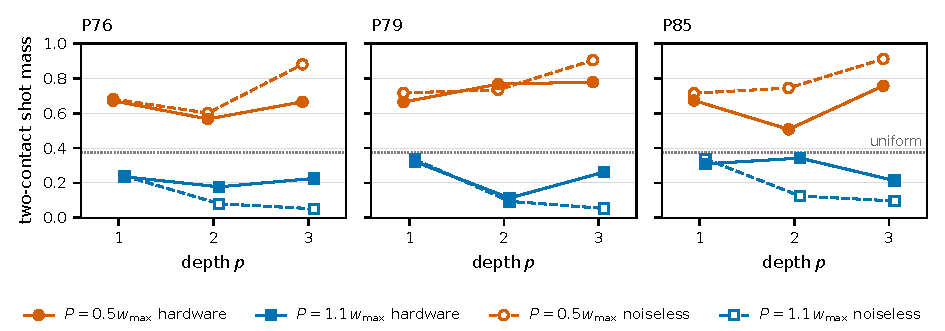
\includegraphics[width=\textwidth]{fig_depth_sweep.pdf}
\caption{Depth sweep on the three 2BM2 subproblems on \texttt{ibm\_marrakesh}: shot mass on the three two-contact strings against depth $p$. Filled markers and solid lines, hardware (mean over five runs of 4096 shots; the sample standard deviations, at most 0.014, are smaller than the markers); open markers and dashed lines, the noiseless circuit. Circles, $P=0.5\,w_{\max}$; squares, $P=1.1\,w_{\max}$. The dotted line is the two-contact mass of uniform sampling over the eight strings, $3/8$.}
\label{fig:sweep}
\end{figure}

\begin{table}[htbp]
\caption{Depth sweep, 2BM2 subproblems on \texttt{ibm\_marrakesh}, five runs of 4096 shots per case. Pair mass is the shot mass on the three two-contact strings; ideal values from the noiseless circuit. Mode gives how many of the five runs had a single-contact string as the most frequent outcome.}
\label{tab:sweep}
\centering
\small
\resizebox{\textwidth}{!}{%
\begin{tabular}{@{}llccccc@{}}
\toprule
Subproblem & Penalty & $p$ & Depth / \texttt{cz} & Pair mass, ideal & Pair mass, hardware & Mode single-contact \\
\midrule
P76 & $0.5\,w_{\max}$ & 1 & 36 / 9 & 0.681 & $0.672 \pm 0.010$ & 0/5 \\
P76 & $0.5\,w_{\max}$ & 2 & 70 / 18 & 0.601 & $0.567 \pm 0.007$ & 0/5 \\
P76 & $0.5\,w_{\max}$ & 3 & 105 / 30 & 0.880 & $0.665 \pm 0.009$ & 0/5 \\
P76 & $1.1\,w_{\max}$ & 1 & 37 / 9 & 0.241 & $0.235 \pm 0.006$ & 5/5 \\
P76 & $1.1\,w_{\max}$ & 2 & 68 / 18 & 0.081 & $0.178 \pm 0.009$ & 5/5 \\
P76 & $1.1\,w_{\max}$ & 3 & 105 / 30 & 0.052 & $0.226 \pm 0.010$ & 5/5 \\
P79 & $0.5\,w_{\max}$ & 1 & 36 / 9 & 0.716 & $0.664 \pm 0.006$ & 0/5 \\
P79 & $0.5\,w_{\max}$ & 2 & 71 / 18 & 0.734 & $0.767 \pm 0.010$ & 0/5 \\
P79 & $0.5\,w_{\max}$ & 3 & 103 / 30 & 0.904 & $0.778 \pm 0.005$ & 0/5 \\
P79 & $1.1\,w_{\max}$ & 1 & 37 / 9 & 0.335 & $0.322 \pm 0.004$ & 5/5 \\
P79 & $1.1\,w_{\max}$ & 2 & 68 / 18 & 0.095 & $0.113 \pm 0.006$ & 5/5 \\
P79 & $1.1\,w_{\max}$ & 3 & 109 / 30 & 0.054 & $0.263 \pm 0.014$ & 5/5 \\
P85 & $0.5\,w_{\max}$ & 1 & 36 / 9 & 0.714 & $0.673 \pm 0.006$ & 0/5 \\
P85 & $0.5\,w_{\max}$ & 2 & 67 / 18 & 0.744 & $0.508 \pm 0.007$ & 0/5 \\
P85 & $0.5\,w_{\max}$ & 3 & 105 / 30 & 0.911 & $0.757 \pm 0.007$ & 0/5 \\
P85 & $1.1\,w_{\max}$ & 1 & 37 / 9 & 0.338 & $0.309 \pm 0.007$ & 5/5 \\
P85 & $1.1\,w_{\max}$ & 2 & 70 / 18 & 0.125 & $0.342 \pm 0.003$ & 5/5 \\
P85 & $1.1\,w_{\max}$ & 3 & 110 / 30 & 0.097 & $0.213 \pm 0.005$ & 5/5 \\
\bottomrule
\end{tabular}}
\end{table}

\subsection{Size study at depth one}
\label{sec:res_size}
Table~\ref{tab:size} and figure~\ref{fig:size} report the $p=1$ circuits on induced subgraphs of each target, each a union of whole protein groups, with the angles re-optimized for every subgraph and penalty on the same $32\times32$ grid. Because every case uses the same optimization procedure, this experiment separates the penalty from the grid confound of section~\ref{sec:res_corr}, and it separates size from both. On 2BM2, where the executed penalty leaves the ground state infeasible at every size, the most frequent string under that penalty is infeasible in all 25 runs at 3, 4, 5, 7 and 8 nodes and feasible in five of five at 10 nodes and two of five at 11, where noise has halved the valid fraction (8.7\% against 20.4\% ideal) and the mode is marginal. Under the corrected penalty the pattern is the mirror image: feasible in all 25 runs up to 8 nodes, then the empty string at 10 and 11 nodes (one of five and none of five feasible). The device follows the noiseless prediction at every size except at the blurred top of the chain. The eleven-node July experiment sat at the one size on this graph where the executed penalty's signature is hidden at depth one.

The 1HSG chain (P52, P51+P52, P136+P51+P52, P139+P51+P52, P136+P139+P51+P52 and all five groups; its seven- and nine-node members are incomparable under inclusion) was run with two off-chain subgraphs added because on this graph the executed penalty leaves the ground state feasible on some subgraphs and infeasible on others: a five-node subgraph, P136+P147+P51, whose ground state is feasible under the executed penalty, and an eight-node subgraph, P136+P139+P147+P52, whose ground state is infeasible. On the chain itself the executed penalty gives an infeasible ground state at 3, 6 and 7 nodes and a feasible one from 9 nodes on. At eight nodes and below the device gave the same answer as on 2BM2 in every run: the most frequent string is infeasible in all 25 executed-penalty runs and feasible in all 25 corrected-penalty runs. The five-node control is the decisive case. Its ground state is feasible under the executed penalty, so the formulation error does not change the answer there, and the depth-one circuit nonetheless placed its mode on an infeasible string in five of five runs, even though among the feasible shots the optimum is over-represented $4.95 \pm 0.16$ times relative to uniform (noiseless 5.49); under the corrected penalty on the same subgraph the mode is feasible in five of five. The depth-one mode follows the penalty-to-weight ratio rather than the location of the ground state, and this is now measured rather than simulated. Above eight nodes the corrected penalty crosses as it did on 2BM2, one size earlier: the mode is infeasible in all fifteen runs at 9, 10 and 11 nodes, as the noiseless circuit predicts, although the ground state is feasible throughout. Under the executed penalty the mode becomes feasible in two of five runs at 9 and 10 nodes and five of five at 11, where the noiseless mode is feasible with probability 0.018, 0.011 and 0.007 (under 80 shots of 4096); on this graph the ground state is also feasible at these sizes, so this arm does not by itself separate size from ground-state location, which is what the five-node control and the 2BM2 chain do. Apart from those two-of-five cases, one case in sixteen disagrees with the noiseless circuit on the feasibility of the mode, and does so in every run: the eight-node control under the corrected penalty, whose noiseless mode is the empty string, with probability 0.047, while the device returned a feasible mode in all five runs: on average 0.021 of its shots fell on the empty string, against 0.042 in the calibration-based simulation, and its most frequent string was the two-contact clique formed by the P136 and P147 contacts in four runs and a single contact in one (section~\ref{sec:res_noise}). The hardware valid fraction tracks the noiseless value to within 0.04 at every size under the executed penalty; under the corrected penalty, which has the larger ideal valid fraction and so the more to lose, it falls below the noiseless value by 0.06 to 0.07 at six and seven nodes and by 0.11 to 0.16 at eight to eleven nodes. The comparison with the calibration-based simulation is in section~\ref{sec:res_noise}.

\begin{figure}[htbp]
\centering
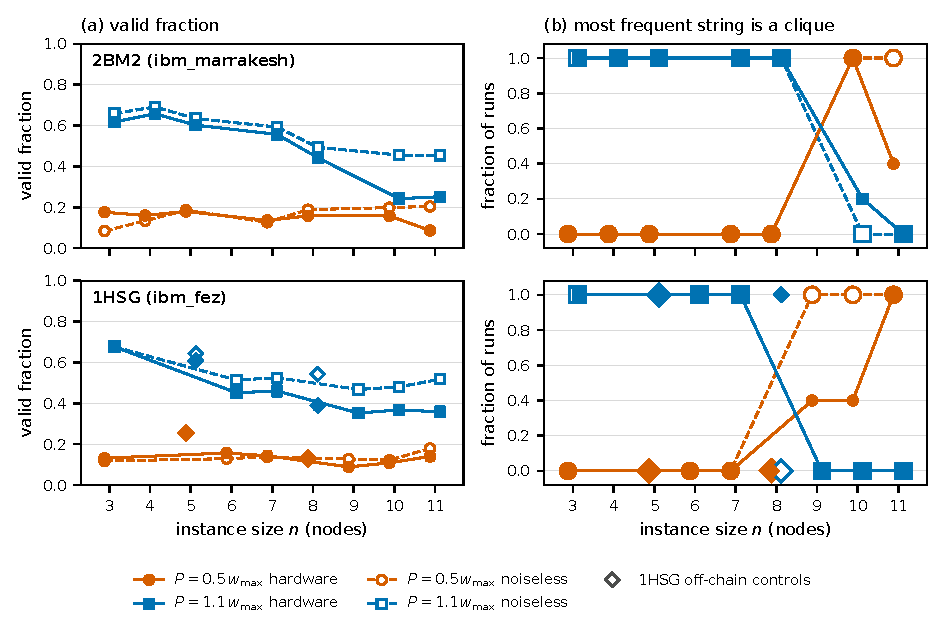
\includegraphics[width=\textwidth]{fig_size_study.pdf}
\caption{Size study at $p=1$ on induced subgraphs that are unions of whole protein groups, with angles re-optimized for every subgraph and penalty; upper row 2BM2 on \texttt{ibm\_marrakesh}, lower row 1HSG on \texttt{ibm\_fez}. (a) Valid fraction; (b) fraction of the five runs whose most frequent string is a clique. Filled markers and solid lines, hardware (mean over five runs of 4096 shots; in (a) the error bars are the sample standard deviations, at most 0.010 for 2BM2 and 0.028 for 1HSG); open markers and dashed lines, the noiseless circuit, whose value in (b) is 0 or 1 and is drawn as a larger ring, so that a filled marker inside a ring indicates agreement. Circles, $P=0.5\,w_{\max}$; squares, $P=1.1\,w_{\max}$; diamonds, the two 1HSG off-chain controls at five and eight nodes, not joined to the chain.}
\label{fig:size}
\end{figure}

\begin{table}[htbp]
\caption{Size study at $p=1$ on induced subgraphs that are unions of whole protein groups: 2BM2 on \texttt{ibm\_marrakesh} (upper block) and 1HSG on \texttt{ibm\_fez} (lower block), five runs of 4096 shots per case, angles from a $32\times32$ grid per case. GS infeasible: whether the global ground state of the case's Hamiltonian is an infeasible string. Mode feasible: runs (of five) in which the most frequent string was a non-empty clique; the noiseless value in parentheses. $^{\dagger}$Off-chain control (section~\ref{sec:res_size}).}
\label{tab:size}
\centering
\small
\resizebox{\textwidth}{!}{%
\begin{tabular}{@{}lccccccc@{}}
\toprule
Groups & $n$ & Penalty & GS infeasible & Valid frac., ideal & Valid frac., hardware & $\rho$, hardware & Mode feasible \\
\midrule
\multicolumn{8}{@{}l}{\textit{2BM2, \texttt{ibm\_marrakesh}}} \\
P79 & 3 & 0.5 & yes & 0.084 & $0.176 \pm 0.003$ & $0.64 \pm 0.05$ & 0/5 (no) \\
P79 & 3 & 1.1 & no & 0.659 & $0.618 \pm 0.006$ & $1.08 \pm 0.02$ & 5/5 (yes) \\
P75+P79 & 4 & 0.5 & yes & 0.134 & $0.160 \pm 0.004$ & $2.16 \pm 0.27$ & 0/5 (no) \\
P75+P79 & 4 & 1.1 & no & 0.692 & $0.658 \pm 0.007$ & $1.89 \pm 0.07$ & 5/5 (yes) \\
P38+P75+P79 & 5 & 0.5 & yes & 0.187 & $0.180 \pm 0.007$ & $1.80 \pm 0.12$ & 0/5 (no) \\
P38+P75+P79 & 5 & 1.1 & no & 0.634 & $0.602 \pm 0.009$ & $1.58 \pm 0.07$ & 5/5 (yes) \\
P75+P76+P79 & 7 & 0.5 & yes & 0.127 & $0.136 \pm 0.007$ & $4.76 \pm 0.53$ & 0/5 (no) \\
P75+P76+P79 & 7 & 1.1 & no & 0.593 & $0.557 \pm 0.010$ & $0.98 \pm 0.04$ & 5/5 (yes) \\
P38+P75+P76+P79 & 8 & 0.5 & yes & 0.189 & $0.158 \pm 0.007$ & $3.75 \pm 0.23$ & 0/5 (no) \\
P38+P75+P76+P79 & 8 & 1.1 & no & 0.493 & $0.443 \pm 0.006$ & $1.60 \pm 0.08$ & 5/5 (yes) \\
P75+P76+P79+P85 & 10 & 0.5 & yes & 0.199 & $0.158 \pm 0.006$ & $0.60 \pm 0.17$ & 5/5 (yes) \\
P75+P76+P79+P85 & 10 & 1.1 & no & 0.456 & $0.242 \pm 0.003$ & $0.59 \pm 0.12$ & 1/5 (no) \\
all five groups & 11 & 0.5 & yes & 0.204 & $0.087 \pm 0.003$ & $2.56 \pm 0.23$ & 2/5 (yes) \\
all five groups & 11 & 1.1 & no & 0.455 & $0.252 \pm 0.008$ & $0.50 \pm 0.15$ & 0/5 (no) \\
\midrule
\multicolumn{8}{@{}l}{\textit{1HSG, \texttt{ibm\_fez}}} \\
P52 & 3 & 0.5 & yes & 0.117 & $0.131 \pm 0.010$ & $1.39 \pm 0.06$ & 0/5 (no) \\
P52 & 3 & 1.1 & no & 0.676 & $0.677 \pm 0.024$ & $1.15 \pm 0.04$ & 5/5 (yes) \\
P136+P147+P51$^{\dagger}$ & 5 & 0.5 & no & 0.252 & $0.257 \pm 0.010$ & $4.95 \pm 0.16$ & 0/5 (no) \\
P136+P147+P51$^{\dagger}$ & 5 & 1.1 & no & 0.644 & $0.608 \pm 0.018$ & $1.60 \pm 0.15$ & 5/5 (yes) \\
P51+P52 & 6 & 0.5 & yes & 0.129 & $0.157 \pm 0.008$ & $2.48 \pm 0.19$ & 0/5 (no) \\
P51+P52 & 6 & 1.1 & no & 0.514 & $0.452 \pm 0.007$ & $1.24 \pm 0.09$ & 5/5 (yes) \\
P136+P51+P52 & 7 & 0.5 & yes & 0.137 & $0.143 \pm 0.020$ & $2.38 \pm 0.15$ & 0/5 (no) \\
P136+P51+P52 & 7 & 1.1 & no & 0.525 & $0.460 \pm 0.028$ & $1.35 \pm 0.10$ & 5/5 (yes) \\
P136+P139+P147+P52$^{\dagger}$ & 8 & 0.5 & yes & 0.124 & $0.133 \pm 0.007$ & $2.08 \pm 0.32$ & 0/5 (no) \\
P136+P139+P147+P52$^{\dagger}$ & 8 & 1.1 & no & 0.543 & $0.389 \pm 0.017$ & $0.88 \pm 0.21$ & 5/5 (no) \\
P139+P51+P52 & 9 & 0.5 & no & 0.127 & $0.089 \pm 0.010$ & $2.67 \pm 0.26$ & 2/5 (yes) \\
P139+P51+P52 & 9 & 1.1 & no & 0.468 & $0.352 \pm 0.016$ & $0.33 \pm 0.10$ & 0/5 (no) \\
P136+P139+P51+P52 & 10 & 0.5 & no & 0.121 & $0.108 \pm 0.009$ & $1.69 \pm 0.26$ & 2/5 (yes) \\
P136+P139+P51+P52 & 10 & 1.1 & no & 0.481 & $0.367 \pm 0.018$ & $0.43 \pm 0.05$ & 0/5 (no) \\
all five groups & 11 & 0.5 & no & 0.179 & $0.140 \pm 0.018$ & $1.33 \pm 0.32$ & 5/5 (yes) \\
all five groups & 11 & 1.1 & no & 0.518 & $0.358 \pm 0.023$ & $0.41 \pm 0.11$ & 0/5 (no) \\
\bottomrule
\end{tabular}}
\end{table}

The eleven-node executed-penalty row of table~\ref{tab:size} is also the parameter-transfer control for the July circuit: same Hamiltonian, angles re-optimized on a finer grid. Its noiseless valid fraction is 0.204 against 0.117 for the July angles, and its optimum concentration $1.48\times$ uniform against $2.21\times$; on hardware, 0.087 against 0.130 and $2.56\times$ against $1.31\times$. Two circuits for one Hamiltonian, both expectation-value optima on their grids, with different feasibility and different optimum concentration. The angles are part of the result.

\subsection{Hardware against calibration-based simulation}
\label{sec:res_noise}
Every executed circuit was simulated with a noise model built from the calibration in force at its execution (section~\ref{sec:setup}). At depth one and up to eight nodes the simulation reproduces the hardware valid fraction and, for three-qubit circuits, the pair mass to within about 0.03 across all penalties, sizes and both devices, with one exception noted below: for example 0.187 against 0.158 at eight nodes on 2BM2, 0.708 against 0.672 for the P79 subproblem, 0.318 against 0.332 for its corrected counterpart, and on 1HSG 0.255 against 0.257 for the five-node control and 0.713 against 0.715 in pair mass for the three-node P52 circuit. Beyond roughly 100 two-qubit gates or depth 100 the two devices part. On \texttt{ibm\_marrakesh} the model under-predicts the degradation: at ten and eleven nodes it gives valid fractions of 0.16 to 0.35 where the device gives 0.09 to 0.25, and at $p=3$ it gives corrected-penalty pair masses of 0.09 to 0.13 where the device gives 0.21 to 0.26. On \texttt{ibm\_fez} it does not: at nine to eleven nodes (103 to 164 \texttt{cz}) the simulated valid fractions are within 0.03 of the device under both penalties (0.350 against 0.358 at eleven nodes under the corrected penalty), and for the corrected depth-three 1HSG subproblems of section~\ref{sec:res_corr} the simulated pair masses, 0.089, 0.109 and 0.124, are within 0.015 of the measured 0.092, 0.118 and 0.121. The exception at small size is the eight-node 1HSG control under the corrected penalty, whose measured valid fraction, 0.389, is 0.08 below the simulated 0.471; the four cases at ten and eleven nodes, executed in the same batch, agree with the model to within 0.015, so the discrepancy is confined to that circuit. It is the same case whose most frequent string disagrees with the noiseless prediction (section~\ref{sec:res_size}): the simulation keeps an infeasible mode in all five simulated runs and places 0.042 of its shots on the empty string, the device 0.021. The July decomposition ran at the depth where the two devices part. The hardware is consistent with its calibration for shallow circuits on both devices; at the depths where the executed decomposition operated it is consistent with its calibration on \texttt{ibm\_fez} and worse than its calibration predicts on \texttt{ibm\_marrakesh}, and the September calibration medians of the two devices (table~\ref{tab:circuits}) are also consistent with \texttt{ibm\_fez} sitting closer to its ideal than \texttt{ibm\_marrakesh} at depth 105 (0.09--0.12 against 0.21--0.26 corrected pair mass).





% =====================================================================
\section{Discussion}
\label{sec:discussion}
%% ~900 words, prose only.
%% 0. FIRST PARAGRAPH: the executed QUBO used P = 0.5 w_max (confirmed from source),
%%    below the P > w_max condition; the 2BM2 Hamiltonian's global argmin is an
%%    invalid 4-node set. At p=1 the ideal circuit still concentrates on the valid
%%    optimum (2.2x uniform-within-valid) so the error is invisible in the output
%%    and AR=100% was guaranteed; at p=3 the subproblem circuits execute the error
%%    (infeasible pairs dominate). Frame as: a formulation error that the standard
%%    metrics cannot detect at shallow depth and that deeper circuits amplify.
%% 1. Why noisy hardware recovers the optimum: the valid-clique subspace is small
%%    (37/2048 and 33/2048, non-empty, measured from the executed circuits); the optimum need only dominate
%%    that subspace, not the full distribution. Do not write 37/2048.
%% 2. 1HSG lower valid-state fraction is a graph property (17 edges / 38 non-edges vs
%%    21 / 34), NOT a hardware property; devices had comparable median cz error.
%%    No cross-target hardware-difficulty comparison of any kind.
%% 3. Why decomposition still needs a classical combiner; ligand-reuse conflicts.
%% 4. Position against Zheng and Chen: Chen's 6-for-18 encoding shows the
%%    one-variable-per-qubit encoding used here is not resource-minimal; discuss
%%    honestly as a limitation and a direction, not as a competing claim.
%% 5. Numbered limitations: two targets at 11 qubits; no error mitigation; two
%%    backends on different days; pharmacophore abstraction limits; unseeded
%%    Vina in the original runs.

The results describe a docking experiment that reported success on two hardware platforms while its formulation was defective, and they locate, with controlled re-executions, the conditions under which such a defect is or is not visible in the output. This section draws out four points and states the limitations.

\subsection{What the reported metrics could and could not detect}
\label{sec:disc_metrics}
The approximation ratio reported in the July campaign, and commonly reported in hardware studies of QAOA on constrained problems, is the weight of the best feasible sample divided by the optimum weight. On a penalty-constrained clique instance of this size that quantity is decided by the size of the feasible set, not by the circuit. With 37 feasible strings and several hundred feasible shots, the optimum appears in the sample with probability $1 - 10^{-6}$ under uniform sampling over the feasible set; the metric would have reported 100\% for a circuit that had learned nothing beyond feasibility. It did report 100\% for a circuit whose Hamiltonian had an infeasible ground state. Two quantities in section~\ref{sec:results} do discriminate. The concentration on the optimum relative to uniform-within-feasible sampling measures whether the circuit prefers the optimum over other cliques, and it is the quantity that moved when the penalty, the size or the angles changed. The feasibility of the most frequent string measures what the circuit is actually optimizing toward, and it is the quantity that exposed the penalty deficiency wherever the deficiency was exposed at all. Neither requires anything beyond the raw counts and the enumerated feasible set; both should accompany any approximation ratio reported on an instance small enough to enumerate.

\subsection{When a formulation error is visible}
\label{sec:disc_visibility}
The executed penalty violated the sufficient condition $P > \max_i w_i$ by a factor of two, and for 2BM2 the ground state of the executed Hamiltonian was an infeasible four-contact set. The three re-execution experiments give a consistent account of when that shows. On three-node instances it shows at every depth from one to three: the most frequent string is a two-contact string in all 45 executed-penalty runs of the sweep and a single contact in all 45 corrected-penalty runs. On the eleven-node 2BM2 instance at depth one it does not show: the most frequent string is feasible and the optimum is over-represented relative to uniform. The size study places the transition on the 2BM2 graph between eight and ten nodes and shows that the corrected penalty crosses in the opposite direction at the same size, from a feasible mode to the empty string, although its ground state is feasible at every size. On the 1HSG graph the corrected penalty crosses between eight and nine nodes, and the executed penalty's mode is infeasible in every run at eight nodes and below, including on a five-node subgraph whose ground state is feasible under that penalty: there the formulation error does not move the optimum, yet the depth-one circuit sampled an infeasible mode in five of five runs on hardware. Across both graphs the depth-one mode follows the penalty-to-weight ratio and the instance size rather than the location of the ground state: at small size the executed penalty gives an infeasible mode whether the ground state is feasible (the five-node 1HSG control) or not, and at large size the mode is feasible over an infeasible ground state on 2BM2 and infeasible over a feasible one under the corrected penalty on both graphs. Ground-state location governs at depth three, where a three-qubit circuit with well-optimized angles concentrates on its ground state: in the noiseless simulation every September depth-three circuit has a two-contact string as its mode under the executed penalty and a single contact under the corrected one, the hardware mode fell in the same class in all 60 depth-three September runs, and in the corrected arm it was the ground state itself for P76, P79 and P139 and the second-heaviest option for P85 and P52 (section~\ref{sec:disc_noise}). Two of the three July 1HSG circuits, whose angles were optimized with fewer restarts on sampled estimates, did not prepare their ground states, and still placed most of their probability on infeasible strings. The July experiment was therefore run at the one combination on its own graph, eleven nodes and depth one, at which its formulation error was invisible in the monolithic output, and its decomposition, which would have exposed the error, reported through a combiner that discarded the exposing mass by construction.

\subsection{The angles are part of the result}
\label{sec:disc_params}
At depth one the expectation-value landscape is nearly degenerate, and expectation-optimal angles from different grids produce circuits with different feasibility behaviour on the same Hamiltonian: 0.40 against 0.57 ideal valid fraction for the corrected 2BM2 Hamiltonian from $30\times30$ and $40\times40$ grids, and, for the executed Hamiltonian, 0.117 against 0.204 between the July angles and the size study's re-optimized ones, with optimum concentrations of $2.21\times$ and $1.48\times$ uniform. The July angles were also transferred from 2BM2 to 1HSG without re-optimization. None of this is unusual practice; the point is that a depth-one QAOA result on a constrained instance is not a property of the Hamiltonian alone, and comparisons across penalties, sizes or papers that do not hold the angle-selection procedure fixed are comparing circuits, not formulations. The corrected monolithic arm of section~\ref{sec:res_corr} is reported with that caveat attached for exactly this reason; the size study, which holds the procedure fixed, is the experiment the penalty conclusion rests on.

\subsection{Noise}
\label{sec:disc_noise}
A noise model built from the calibration in force at execution reproduces the hardware to within about 0.03 in valid fraction and pair mass for every circuit up to eight nodes at depth one and every three-qubit circuit at depth one, on both devices and both penalties, with a single exception (the eight-node 1HSG control under the corrected penalty, 0.08 below the model). Beyond roughly 100 two-qubit gates the two devices part. On \texttt{ibm\_marrakesh} the model under-predicts the degradation, by a factor of about two in valid fraction at ten and eleven nodes and by about 0.15 in pair mass at depth 105; on \texttt{ibm\_fez} it reproduces the device to within 0.03 at nine to eleven nodes and to within 0.015 in pair mass for the depth-three corrected subproblems. Whether a calibration-based model is adequate at the depth of the July decomposition is therefore a property of the device and the period, not of the depth alone. The executed decomposition ran at that depth on both devices, and the sweep on \texttt{ibm\_marrakesh} shows the consequence there: the ideal separation between penalties grows by about 0.4 from depth one to three while the measured separation grows by 0.0 to 0.2, so that on that device about half of what depth adds in the ideal is lost to noise by depth 105. The difference between the two targets' July optimum concentrations, which a reader of the July record would have been tempted to interpret as a property of the instances, is a valid-fraction effect of noise on the deeper 1HSG circuit.

One further point bears on the corrected-penalty results at depth one, whose mode is the empty string. That is a property of the circuit, not of the device. The noiseless corrected circuits give the empty string a probability of 0.058 and 0.093 (monolithic 2BM2 and 1HSG) and 0.039 and 0.064 (the eleven-node size-study circuits); the device gives it less, $0.026 \pm 0.002$, $0.047 \pm 0.002$, $0.019 \pm 0.002$ and $0.047 \pm 0.010$; and the calibration model accounts for part of the reduction in the first three cases (0.038, 0.059, 0.027) and slightly more than all of it in the fourth (0.041). Noise moves mass away from the empty string, toward the uniform background, not toward it.

Run-to-run scatter within a calibration is not shot-noise limited. For the optimum's shot count it is (section~\ref{sec:res_july}), but the five-run sample standard deviation of the valid fraction (of the pair mass in the sweep) exceeds the binomial value by up to about 1.3 times in the September 2BM2 size chain, 2 times in the sweep and the corrected monolithic circuits, 3.6 times in the October 1HSG size chain, 4 times in the July 2BM2 monolithic runs and 4.4 times in the corrected 1HSG subproblems, so the five runs sample short-term drift as well as shot noise. Nothing here speaks to drift across calibrations beyond the one set of section~\ref{sec:setup}.

A related observation concerns near-degenerate subproblems. Three of the six corrected three-node subproblems have two options within 3\% in weight, P79 (0.953, 0.982), P85 (0.980, 1.000) and P51 (0.923, 0.923, exactly degenerate), and a fourth, P52, has two within 7\% (0.935, 1.000) whose ideal probabilities at depth three nonetheless differ by only 0.008 (0.457 against 0.465). P79 chose the heavier option in five of five runs, P85 the lighter in five of five, P52 the lighter in five of five, and P51, whose two options have identical ideal probability (0.394 each), placed its mode on node 6 in three runs and node 7 in two. Shot noise at 4096 shots cannot separate options whose ideal probabilities differ by 0.004 or 0.008, so a choice reproduced in five of five runs indicates a systematic device asymmetry, a qubit-specific gate or readout bias, that selects one option; the exact tie, by contrast, split three to two, as shot noise on an exact tie would. Near-ties on hardware are resolved by the device rather than by the Hamiltonian, here twice against the optimum, and an exact tie is not resolved at all.

\subsection{Limitations}
\label{sec:disc_limits}
The study covers two targets, eleven nodes, depths one to three and two processors of one family, without error mitigation. The absolute scale of the node weights is not recoverable from the executed circuits and the docking runs that produced them were not seeded; the relative weights, the edge sets and the optima are exact and are given in full in the repository, and a seeded re-docking was not performed. The eleven-node instances are small enough to enumerate, so nothing in the paper bears on quantum advantage, and the classical enumeration is the reference throughout. The corrected monolithic arm is confounded by grid resolution, as stated. The feasibility of the most frequent string is a weak statistic where the noiseless distribution is nearly flat, as it is at nine to eleven nodes under the executed penalty (mode probabilities below 0.02), and the blurred top of both size chains should be read with that in mind; the valid fraction and the optimum concentration are reported alongside it for that reason. Finally, the July analysis code was not preserved and its summaries were wrong in several places; every quantity in this paper was recomputed from the retrieved counts and the submitted circuits, and the reconstruction method is described so that the same check can be applied to other hardware records.

% =====================================================================
\section{Conclusion and future work}
\label{sec:conclusion}

This paper examined a QAOA docking experiment on IBM Heron processors whose formulation carried a penalty below the condition needed for a feasible ground state, and asked what the reported hardware quantities could reveal about that. Reconstructing the instances from the submitted circuits showed the defect directly; recomputing the statistics from the raw counts showed that the reported approximation ratio of 100\% was guaranteed by the size of the feasible set and carried no information; and three re-execution experiments on the same graphs and devices established the conditions under which the defect is visible in the output. It is visible at every depth on three-node instances, invisible at depth one on the eleven-node 2BM2 instance, and the transition between the two lies between eight and ten nodes on the 2BM2 graph and above eight nodes on the 1HSG graph, with the corrected penalty crossing in the opposite direction at the same sizes. At depth one the most frequent string follows the penalty-to-weight ratio and the instance size rather than the location of the ground state, as measured directly on a five-node 1HSG subgraph whose ground state is feasible under the executed penalty and whose sampled mode was infeasible in every run; at depth three, with well-optimized angles, it follows the ground state. The expectation-optimal angles are part of the result, since angles from different grids on one Hamiltonian give different feasibility behaviour, and a calibration-based noise model accounts for both devices up to about 100 two-qubit gates and, beyond that, for \texttt{ibm\_fez} but not for \texttt{ibm\_marrakesh}, whose degradation it under-predicts.

The practical recommendations are short. On any instance small enough to enumerate, report the concentration on the optimum relative to uniform sampling within the feasible set and the feasibility of the most frequent string alongside the approximation ratio, since the ratio alone cannot detect an infeasible ground state at realistic shot counts. Check the penalty condition against the weight table before execution, and check it again on any subproblem produced by decomposition, whose ground state is the first thing a shallow circuit on three qubits will find. Hold the angle-selection procedure fixed across every comparison, and record it. Where a decomposition is recombined classically, report the subproblem distributions themselves, because a combiner that reads only supports will return the classical answer regardless of what the circuits did.

Future work follows from the limitations. A seeded re-docking will restore the absolute weight scale and the provenance of the pharmacophore selection. Larger targets, at fifteen to twenty nodes, would test whether the transition, which lies above eight nodes on both graphs here, scales with the feasible fraction as the uniform-sampling argument predicts. And the same reconstruction, from submitted circuits and retrieved counts, can be applied to other published hardware records of constrained QAOA, which is the audit this paper argues such results need.

% =====================================================================
% Unnumbered back matter (iopjournal macros)
% =====================================================================

\ack{This work used IBM Quantum services through the IBM Quantum Open Plan. The views expressed are those of the author and do not reflect the official policy or position of IBM or the IBM Quantum team. The manuscript text and the analysis, submission and consistency-check scripts were drafted with the assistance of Claude (Anthropic), which also proposed the design of the September re-execution experiments and the reconstruction method, under the author's direction; the author ran all docking and hardware executions, verified every reported number against the raw job records, and is responsible for the content.}

\funding{This work received no external funding.}
%% TODO confirm: LightWater Capital resources were not used for this work.

\roles{Suriya Narayanan Rajavel: Conceptualization, Methodology, Software, Investigation, Validation, Formal analysis, Data curation, Visualization, Writing -- original draft, Writing -- review \& editing.}

\data{The job identifiers of all 340 submitted circuits (60 from July 2026 and 280 from September 2026), the calibration snapshots in force at each execution, the reconstructed instances, the analysis scripts and the corrected results files are available at \todo{GitHub repository URL} under the MIT licence (code) and the CC BY 4.0 licence (data). Raw shot counts of every executed job are included in the repository and can also be retrieved from IBM Quantum with the listed job identifiers.}

\suppdata{Per-run measurement tables for all 340 jobs, the executed edge sets and relative weights, the calibration snapshots in force at each execution and the submitted-circuit audit output are provided in the repository cited above.}

%% AI-assistance statement: in the acknowledgements above and, in the same words, in the cover letter.

\section*{References}
%% TODO confirm iopart-num renders correctly under iopjournal; the class ships no .bst and the back-matter macros (\ack, \data, \roles) are iopjournal-only
\bibliographystyle{iopart-num}
\bibliography{references}

\end{document}
